%--------------------------------------------------------------------------------------
% Dokumentum formátuma [Document format]
%--------------------------------------------------------------------------------------

\documentclass[12pt,a4paper,oneside]{report}             % Egyoldalas [Single-side]
%\documentclass[12pt,a4paper,twoside,openright]{report}  % Kétoldalas [Duplex]


%--------------------------------------------------------------------------------------
% Csomagok inicializálása [Initializing packages]
%--------------------------------------------------------------------------------------
\usepackage{ifthen} % Used in macros

\usepackage[english,magyar]{babel} % Language support
\usepackage{geometry}
\usepackage{amsfonts,amsmath,amssymb} % Mathematical symbols
\usepackage{microtype} % Imrovements to typesetting
\usepackage{setspace} % For setting line spacing
\usepackage{cmap} % Enables more advenced text copying from the PDF document 
\usepackage{sectsty} % Section heading styling
\usepackage{pdfpages}

\usepackage[unicode]{hyperref} % For hyperlinks in the generated document
\usepackage{booktabs} % For publication quality tables for LaTeX
\usepackage{graphicx} % For figure sizing
\usepackage[hang]{caption}
\usepackage{xcolor} % For code coloring in listings
\usepackage{listings} % For source code snippets
\usepackage[amsmath,thmmarks]{ntheorem} % Theorem-like environments

\usepackage[numbers]{natbib} % Bibliography

%\usepackage{fancyhdr} % For easy to use headers and footers

% thanks to http://tex.stackexchange.com/a/47579/71109
\usepackage{ifxetex}
\usepackage{ifluatex}
\newif\ifxetexorluatex % a new conditional starts as false
\ifnum 0\ifxetex 1\fi\ifluatex 1\fi>0
   \xetexorluatextrue
\fi

\ifxetexorluatex
  \usepackage{fontspec}
  % Palatino clone font (Tex Gyre Pagella) for text and math
  \usepackage{newpxmath}
  \setmainfont[Ligatures=TeX]{TeX Gyre Pagella}
\else
  \usepackage[T1]{fontenc}
  \usepackage[utf8]{inputenc}
  %\usepackage[lighttt]{lmodern} % Advanced version of the Computer Modern font
  % Palatino clone font (Tex Gyre Pagella) for text and math
  \usepackage{tgpagella, newpxmath}
\fi



%--------------------------------------------------------------------------------------
% Dokumentum nyelve [Language]
%--------------------------------------------------------------------------------------

%--------------------------------------------------------------------------------------
% Elnevezések
%--------------------------------------------------------------------------------------
\newcommand{\bme}{Budapesti Műszaki és Gazdaságtudományi Egyetem}
\newcommand{\gpk}{Gépészmérnöki Kar}

\newcommand{\bmeatt}{Anyagtudomány és Technológia Tanszék}
\newcommand{\bmeara}{Áramlástan Tanszék}
\newcommand{\bmeenergia}{Energetikai Gépek és Rendszerek Tanszék}
\newcommand{\bmeepget}{Épületgépészeti és Gépészeti Eljárástechnika Tanszék}
\newcommand{\bmegtharom}{Gép- és Terméktervezés Tanszék}
\newcommand{\bmemanuf}{Gyártástudomány és -technológia Tanszék}
\newcommand{\bmehds}{Hidrodinamikai Rendszerek Tanszék}
\newcommand{\bmemogi}{Mechatronika, Optika és Gépészeti Informatika Tanszék}
\newcommand{\bmemm}{Műszaki Mechanika Tanszék}
\newcommand{\bmept}{Polimertechnika Tanszék}

\newcommand{\keszitette}{Készítette}
\newcommand{\konzulens}{Konzulens}
\newcommand{\temavezeto}{Témavezető}

\newcommand{\selectbsc}{
  \newcommand{\gpkmunkatipus}{Szakdolgozat}       % Dokumentum típusa [Document type]
  \newcommand{\gpkmunkatipusHU}{Szakdolgozat}     % Dokumentum típusa HU
  \newcommand{\gpkmunkatipusok}{Szakdolgozatok}   % többesszámban
  \newcommand{\gpkmunkatipustHU}{Szakdolgozatot}  % tárgyraggal
}
\newcommand{\selectmsc}{
  \newcommand{\gpkmunkatipus}{Diplomaterv}        % Dokumentum típusa [Document type]
  \newcommand{\gpkmunkatipusHU}{Diplomaterv}      % Dokumentum típusa HU
  \newcommand{\gpkmunkatipusok}{Diplomatervek}    % többesszámban
  \newcommand{\gpkmunkatipustHU}{Diplomatervet}   % tárgyraggal
}

\newcommand{\tdk}{TDK dolgozat}
\newcommand{\bsconlab}{BSc Önálló laboratórium}
\newcommand{\msconlabi}{MSc Önálló laboratórium 1.}
\newcommand{\msconlabii}{MSc Önálló laboratórium 2.}

\newcommand{\szerzoijog}{Szerzői jog}

\newcommand{\pelda}{Példa}
\newcommand{\definicio}{Definíció}
\newcommand{\tetel}{Tétel}

\newcommand{\jelolesek}{Jelölések jegyzéke}
\newcommand{\eloszo}{Előszó}
\newcommand{\bevezetes}{Bevezetés}
\newcommand{\koszonetnyilvanitas}{Köszönetnyilvánítás}
\newcommand{\osszefoglalas}{Összefoglalás}
\newcommand{\summary}{Summary}
\newcommand{\fuggelek}{Függelék}
\newcommand{\melleklet}{Mellékletek}

% Opcionálisan átnevezhető címek
\addto\captionsmagyar{%
\renewcommand{\listfigurename}{Illusztrációk jegyzéke}
%\renewcommand{\listtablename}{Saját táblázatjegyzék cím}
%\renewcommand{\bibname}{Saját irodalomjegyzék név}
}

\newcommand{\authorName}{\authorFamilyName{} \authorGivenName}
\newcommand{\consulentA}{\consulentATitle\consulentAFamilyName{} \consulentAGivenName}
\newcommand{\consulentB}{\consulentBTitle\consulentBFamilyName{} \consulentBGivenName}
\newcommand{\consulentC}{\consulentCTitle\consulentCFamilyName{} \consulentCGivenName}
\newcommand{\supervisor}{\supervisorTitle\supervisorFamilyName{}
\supervisorGivenName}

\newcommand{\selectthesislanguage}{\selecthungarian}
\newcommand{\selectforeignlanguage}{\selectenglish}

\bibliographystyle{huplain}

\def\lstlistingname{lista}

\newcommand{\appendixletter}{6} % a fofejezet-szamlalo az angol ABC 6. betuje (F) lesz
\newcommand{\annexletter}{13} % M betű
 % Beállítások magyar nyelvű dolgozathoz

% Megjegyzés: 
%         Ez a beállítás az automatikusan létrehozott címek, hivatkozások
%         nyelvét adja meg, valamint a nyelvre jellemző behúzási távolságot
%         használja a bekezdések elején.
%
% Note: 
%         This setting controls the language of generated titles and citations,
%         moreover the paragraph indentation.


%--------------------------------------------------------------------------------------
% Preambulum (LaTeX beállítások, makrók) [Preamble (LaTeX settings)]
%--------------------------------------------------------------------------------------
%--------------------------------------------------------------------------------------
% Page layout setup
%--------------------------------------------------------------------------------------
% we need to redefine the pagestyle plain
% another possibility is to use the body of this command without \fancypagestyle
% and use \pagestyle{fancy} but in that case the special pages
% (like the ToC, the References, and the Chapter pages)remain in plane style

\pagestyle{plain}
\geometry{inner=30mm, outer=20mm, top=20mm, bottom=30mm}


%--------------------------------------------------------------------------------------
% Text and paragraph styling
%--------------------------------------------------------------------------------------

\sectionfont{\Large\upshape\bfseries}  % Section title font
\subsectionfont{\Large\itshape\mdseries}
\subsubsectionfont{\large\itshape\mdseries}
\setcounter{secnumdepth}{3}             % Section numbering depth

\sloppy                                 % Prevent text from spilling over the margin
\widowpenalty=10000 \clubpenalty=10000  % Prevent widow and oprhan rows
\def\hyph{-\penalty0\hskip0pt\relax}    % Enable hyphenation

\onehalfspacing                         % 1.5x Line spacing

% Text setup for Hungarian text
\newcommand{\selecthungarian}{
	\selectlanguage{magyar}
	\setlength{\parindent}{2em}			% Paragraph indentation
	\setlength{\parskip}{5pt}			% Paragraph spacing
	\frenchspacing
}

% Text setup for English text
\newcommand{\selectenglish}{
	\selectlanguage{english}
	\setlength{\parindent}{0em}
	\setlength{\parskip}{8pt}
	\nonfrenchspacing
}

%--------------------------------------------------------------------------------------
% Setup hyperref package
%--------------------------------------------------------------------------------------
\hypersetup{
    % bookmarks=true,            % show bookmarks bar?
    unicode=true,                % non-Latin characters in Acrobat's bookmarks
    pdfnewwindow=true,           % links in new window
    colorlinks=true,             % false: boxed links; true: colored links
    linkcolor=black,             % color of internal links
    citecolor=black,             % color of links to bibliography
    filecolor=black,             % color of file links
    urlcolor=black               % color of external links
}

%--------------------------------------------------------------------------------------
% Apply variables
%--------------------------------------------------------------------------------------
% This command is called in the main tex file and uses variables set there.
\newcommand{\applyvariables}{
	\author{\authorName}
	\title{\thesisTitle}

	\hypersetup{
		pdftitle={\thesisTitle},     % title
		pdfauthor={\authorName},     % author
		pdfsubject={\gpkmunkatipus}, % subject of the document
		pdfkeywords={\keywords},     % list of keywords (separate then by comma)
		pdfproducer={\authorName},   % producer of the document (organization)
		pdfcreator={LaTeX}           % creator of the document (application)
	}
}

%--------------------------------------------------------------------------------------
% Set up listings
%--------------------------------------------------------------------------------------
\definecolor{lightgray}{rgb}{0.95,0.95,0.95}
\lstset{
	basicstyle=\scriptsize\ttfamily, % print whole listing small
	keywordstyle=\color{black}\bfseries, % bold black keywords
	identifierstyle=, % nothing happens
	% default behavior: comments in italic, to change use
	% commentstyle=\color{green}, % for e.g. green comments
	stringstyle=\scriptsize,
	showstringspaces=false, % no special string spaces
	aboveskip=3pt,
	belowskip=3pt,
	backgroundcolor=\color{lightgray},
	columns=flexible,
	keepspaces=true,
	escapeinside={(*@}{@*)},
	captionpos=b,
	breaklines=true,
	frame=single,
	float=!ht,
	tabsize=2,
	literate=*
		{á}{{\'a}}1	{é}{{\'e}}1	{í}{{\'i}}1	{ó}{{\'o}}1	{ö}{{\"o}}1	{ő}{{\H{o}}}1	{ú}{{\'u}}1	{ü}{{\"u}}1	{ű}{{\H{u}}}1
		{Á}{{\'A}}1	{É}{{\'E}}1	{Í}{{\'I}}1	{Ó}{{\'O}}1	{Ö}{{\"O}}1	{Ő}{{\H{O}}}1	{Ú}{{\'U}}1	{Ü}{{\"U}}1	{Ű}{{\H{U}}}1
}


%--------------------------------------------------------------------------------------
% Set up theorem-like environments
%--------------------------------------------------------------------------------------
% Using ntheorem package -- see http://www.math.washington.edu/tex-archive/macros/latex/contrib/ntheorem/ntheorem.pdf

\theoremstyle{plain}
\theoremseparator{.}
\newtheorem{example}{\pelda}

\theoremseparator{.}
%\theoremprework{\bigskip\hrule\medskip}
%\theorempostwork{\hrule\bigskip}
\theorembodyfont{\upshape}
\theoremsymbol{{\large \ensuremath{\centerdot}}}
\newtheorem{definition}{\definicio}

\theoremseparator{.}
%\theoremprework{\bigskip\hrule\medskip}
%\theorempostwork{\hrule\bigskip}
\newtheorem{theorem}{\tetel}


%--------------------------------------------------------------------------------------
% Some new commands and declarations
%--------------------------------------------------------------------------------------
\newcommand{\code}[1]{{\upshape\ttfamily\scriptsize\indent #1}}
\newcommand{\doi}[1]{DOI: \href{http://dx.doi.org/\detokenize{#1}}{\raggedright{\texttt{\detokenize{#1}}}}} % A hivatkozások közt így könnyebb DOI-t megadni.

\DeclareMathOperator*{\argmax}{arg\,max}
%\DeclareMathOperator*[1]{\floor}{arg\,max}
\DeclareMathOperator{\sign}{sgn}
\DeclareMathOperator{\rot}{rot}


%--------------------------------------------------------------------------------------
% Setup captions
%--------------------------------------------------------------------------------------
\captionsetup[figure]{
	width=.75\textwidth,
	aboveskip=10pt}

\renewcommand{\captionlabelfont}{\it}
\renewcommand{\captionfont}{\footnotesize\it}

%--------------------------------------------------------------------------------------
% Hyphenation exceptions
%--------------------------------------------------------------------------------------
\hyphenation{Shakes-peare Mar-seilles ár-víz-tű-rő tü-kör-fú-ró-gép}


%--------------------------------------------------------------------------------------
% Command to exclude tables and images in the annex from the List of Figures/Tables
%--------------------------------------------------------------------------------------
\newcommand{\excludeFromLocAndLot}{
	% Redefine \addcontentsline to be silent when printing loc or toc entries
	\let\svaddcontentsline\addcontentsline
	\renewcommand\addcontentsline[3]{
		\ifthenelse{\equal{##1}{lof}}{}{
			\ifthenelse{\equal{##1}{lot}}{}{
				\svaddcontentsline{##1}{##2}{##3}
			}
		}
	}
}


%--------------------------------------------------------------------------------------
% Munkatípus [Thesis type]
%--------------------------------------------------------------------------------------

\selectmsc   % Diplomaterv [Master's]


%--------------------------------------------------------------------------------------
% Változók beállítása [Setting variables]
%--------------------------------------------------------------------------------------

%TODO Állítsd be az alábbi változókat [Set these variables]

% Szerző [Author]
\def\authorFamilyName{Bodnár}
\def\authorGivenName{Bence Tibor}
\def\neptun{H2JC4M}

% Konzulens 1 [Consulent 1]
\def\consulentATitle{}
\def\consulentAFamilyName{Dudás}
\def\consulentAGivenName{Dávid}
\def\consulentARank{óraadó}

% Konzulens 2 [Consulent 2], ha nincs hagyd üresen
\def\consulentBTitle{}
\def\consulentBFamilyName{}
\def\consulentBGivenName{}
\def\consulentBRank{}

% Konzulens 3 [Consulent 3], ha nincs hagyd üresen 
\def\consulentCTitle{}
\def\consulentCFamilyName{}
\def\consulentCGivenName{}
\def\consulentCRank{}

% Témavezető
\def\supervisorTitle{dr.~}
\def\supervisorFamilyName{Budai}
\def\supervisorGivenName{Csaba}
\def\supervisorRank{adjunktus}

% Dolgozat címe [Thesis title]
\def\thesisTitle{Hat szabadsági fokú telemanipulátor fejlesztése sebészeti eszközök számára}

% Kulcsszavak (a PDF-be) [Keywords (to PDF)]
\def\keywords{mechatronika, szabályozástechnika, robotika, ipar 4.0}

% Tanszék [Department]
\def\department{\bmemogi}

%TODO Cseréld le a figures/tanszek_logo.pdf képet a tanszéked logójára!
%     [Replace figures/tanszek_logo.pdf with the logo of your department]

% Elzártan kezelendő dolgozat [Restricted access]
%TODO Töltsd ki a korlátozás lejártának dátumát! 
%     [Fill in the end date of the restriction]
\def\endOfRestrictedAccess{... év ... hónap ... nap}


% Változók beállítása a PDF fájlhoz [Apply variables for the PDF file]
\applyvariables


%--------------------------------------------------------------------------------------
% Dokumentum törzse [Document body]
%--------------------------------------------------------------------------------------

\begin{document}

\pagenumbering{gobble}
\selectthesislanguage

% Címoldal [Titlepage]
\hypersetup{pageanchor=false}

%--------------------------------------------------------------------------------------
% Szennycímoldal [Cover title page]
%--------------------------------------------------------------------------------------

\clearpage
\begin{center}
\MakeUppercase{\authorName}\\[0.1cm]
\MakeUppercase{\gpkmunkatipus}\\[0.1cm]
\end{center}
\thispagestyle{empty}

%--------------------------------------------------------------------------------------
% Sorozatcímoldal [Series title page]
%--------------------------------------------------------------------------------------
\clearpage
\begin{center}


\includegraphics[width=60mm,keepaspectratio]{figures/bme_logo.pdf}\\
\vspace{0.3cm}
\MakeUppercase{\textbf{\bme}}\\[0.1cm]
\MakeUppercase{\textmd{\gpk}}\\[0.1cm]
\MakeUppercase{\textmd{\department}}\\[0.8cm]


\includegraphics[height=40mm,keepaspectratio]{figures/tanszek_logo}\\[0.5cm]
\MakeUppercase{\gpkmunkatipusok}

\end{center}
\thispagestyle{empty}

%--------------------------------------------------------------------------------------
% Címoldal [Title page]
%--------------------------------------------------------------------------------------
\begin{titlepage}
\begin{center}

\includegraphics[width=60mm,keepaspectratio]{figures/bme_logo.pdf}\\
\vspace{0.3cm}
\MakeUppercase{\textbf{\bme}}\\[0.1cm]
\MakeUppercase{\textmd{\gpk}}\\[0.1cm]
\MakeUppercase{\textmd{\department}}

\vspace{4.0cm}
{\huge \textsc{\authorName}}\\[0.8cm]
{\huge \MakeUppercase{\gpkmunkatipus}}\\[0.8cm]
{\Large \thesisTitle}

\vspace{3.0cm}

{
	\renewcommand{\arraystretch}{0.85}
	\begin{tabular}{ll}
	 \makebox[7cm][l]{\konzulens:} & \makebox[7cm][l]{\temavezeto:} \\
	 \noalign{\smallskip}
	 \makebox[7cm][l]{\hspace{1cm}\emph{\consulentA}} & \makebox[7cm][l]{\hspace{1cm}\emph{\supervisor}} \\
	 \makebox[7cm][l]{\hspace{1cm}\consulentARank} & \makebox[7cm][l]{\hspace{1cm}\supervisorRank} \\
	 \\
	 \makebox[7cm][l]{\hspace{1cm}\emph{\consulentB}} & \\
	 \makebox[7cm][l]{\hspace{1cm}\consulentBRank} & \\
	 \\
	 \makebox[7cm][l]{\hspace{1cm}\emph{\consulentC}} & \\
	 \makebox[7cm][l]{\hspace{1cm}\consulentCRank} & \\
	 
	\end{tabular}
}

\vfill
{\Large Budapest, \the\year.}
\end{center}
\end{titlepage}
\hypersetup{pageanchor=false}
\thispagestyle{empty}
  % Szakdolgozat/Diplomaterv címlap [Thesis]

\selectlanguage{magyar}
\pagenumbering{gobble}
\selecthungarian
%--------------------------------------------------------------------------------------
% Copyrightoldal
%--------------------------------------------------------------------------------------
\begin{flushleft}
\szerzoijog{} {\textcopyright} \authorName, \the\year.
\end{flushleft}

\vfill
\clearpage
\thispagestyle{empty} % an empty page

\selectthesislanguage
               % Nyílt kezelésű [Open access]



% Feladatkiírás [Project page]
%TODO A nyomtatott verzóban ne szerepeljen! [Remove before printing]
%--------------------------------------------------------------------------------------
% Feladatkiiras (a tanszeken atveheto, kinyomtatott valtozat)
%--------------------------------------------------------------------------------------
\begin{center}
\large
\textbf{FELADATKIÍRÁS}\\
\end{center}
\thispagestyle{empty}

A feladatkiírást a tanszéki adminisztrációban lehet átvenni, és a leadott munkába eredeti, tanszéki pecséttel ellátott és a tanszékvezető által aláírt lapot kell belefűzni (ezen oldal \emph{helyett}, ez az oldal csak útmutatás). Az elektronikusan feltöltött dolgozatban már nem kell beleszerkeszteni ezt a feladatkiírást.



% Nyilatkozatok [Declarations]
\selectlanguage{magyar}
\selecthungarian
\pagenumbering{roman}
\setcounter{page}{6}
\cleardoublepage % duplexnél páratlan oldalon legyen
%--------------------------------------------------------------------------------------
% Nyilatkozatok
%--------------------------------------------------------------------------------------
\begin{center}
\section*{NYILATKOZAT}
\end{center}

\vspace{0.5cm}

\begin{center}
\emph{Nyilatkozat az önálló munkáról}
\end{center}
Alulírott,  \emph{\authorFamilyName{} \authorGivenName} (\neptun), a Budapesti Műszaki és Gazdaságtudományi Egyetem hallgatója, büntetőjogi és fegyelmi felelősségem tudatában kijelentem és sajátkezű aláírásommal igazolom, hogy ezt a \MakeLowercase{\gpkmunkatipustHU} meg nem engedett segítség nélkül, saját magam készítettem, és dolgozatomban csak a megadott forrásokat használtam fel. Minden olyan részt, melyet szó szerint vagy azonos értelemben, de átfogalmazva más forrásból átvettem, egyértelműen, a hatályos előírásoknak megfelelően, a forrás megadásával megjelöltem.

\begin{flushleft}
Budapest, \today
\end{flushleft}

\begin{flushright}
 \makebox[7cm]{\rule{6cm}{.4pt}}\\
 \makebox[7cm]{\emph{hallgató}}
\end{flushright}


\vfill
\clearpage

\selectthesislanguage

\newcounter{romanPage}
\setcounter{romanPage}{\value{page}}
\stepcounter{romanPage}


\selectthesislanguage
% Tartalomjegyzék [Table of Contents]
\setcounter{tocdepth}{3}  % Tartalomjegyzék mélysége [ToC depth]
\tableofcontents\vfill


% Ábrák és táblázatok jegyzéke [List of Figures, Tables]
%TODO Kommenteld ki, ha használni szeretnéd. [Uncomment to use]
%\listoffigures\addcontentsline{toc}{chapter}{\listfigurename}   % Ábrák jegyzéke - opcionális
%\listoftables\addcontentsline{toc}{chapter}{\listtablename}     % Táblázatok jegyzéke - opcionális


% Előszó [Preface]
%----------------------------------------------------------------------------
\chapter*{\eloszo}\addcontentsline{toc}{chapter}{\eloszo}
%----------------------------------------------------------------------------

Az előszó legtöbbször személyes hangú, eligazító jellegű írás, amely a mű megírásának okairól, születésének körülményeiről szól. Az előszó nem szerves része a főszövegnek, hanem annak kiegészítése.
Ugyancsak az előszóban fejtheti ki a szerző a mű megértéséhez szükséges szempontokat, a követett módszereket, utalhat a fontosabb előzményekre és szakirodalomra.
Az előszó ne legyen terjedelmes.


Jelen dokumentum egy diplomaterv-sablon, amely formai keretet ad a BME Gépészmérnöki Karán végző hallgatók által elkészítendő szakdolgozatnak és diplomatervnek. A sablon használata opcionális. Ez a sablon \LaTeX~alapú, a \emph{TeXLive} \TeX-implementációval és a PDF-\LaTeX~fordítóval működőképes.
A sablon forrása a Mechatronika Szakosztály GitHub tárhelyén\footnotemark{} elérhető. Amennyiben hibát találtál, vagy észrevételed, javaslatod lenne, kérlek ott jelezd.

\footnotetext{\url{https://github.com/MechatronikaSzakosztaly/bme-gpk-thesis-latex}}

\begin{center}
    $\thicksim \; \thicksim \; \thicksim$
\end{center}


\subsubsection*{Köszönetnyilvánítás}
\emph{Szeretnék köszönetet mondani témavezetőmnek, Dr. Budai Csabának és a konzulensemnek Dudás Dávidnak a több féléves munkájáért. Szeretném megköszönni Dr. Bodnár Tibor, Bodnárné Dr. Gyarmathy Dórának és Dr. Gyarmathy Miklósnénak a támogatást és a lektorálást. Szeretnék köszönetet mondani Dr. Kiss Rita tanészékvezető asszonynak és tanészékének a támogatásért. Szeretném megköszönni az Orvostechnika Szakosztály tagjainak a projektben vállalt kisebb feladatokban nyújtott segítséget, illetve a lehetőséget, hogy ezzel a projekttel hozzájárulhattam a Szakosztály életéhez.} 


\vspace{0.5cm}

\begin{flushleft}
{Budapest, \today}
\end{flushleft}

\begin{flushright}
\emph{\authorName}
\end{flushright}

\vfill



% Jelölések jegyzéke [Table of Symbols]
\newcommand{\tss}{\textsuperscript}     % tss = felső index
%----------------------------------------------------------------------------
\chapter*{\jelolesek}\addcontentsline{toc}{chapter}{\jelolesek}
%----------------------------------------------------------------------------

A táblázatban a többször előforduló jelölések magyar és angol nyelvű elnevezése, 
valamint a fizikai mennyiségek esetén annak mértékegysége található. Az egyes 
mennyiségek jelölése – ahol lehetséges – megegyezik hazai és a nemzetközi 
szakirodalomban elfogadott jelölésekkel. A ritkán alkalmazott jelölések 
magyarázata első előfordulási helyüknél található.

%~~~~~~~~~~~~~~~~~~~~~~~~~~~~~~~~~~~~~~~~~~~~~~~~~~~~~~~~~~~~~~~~~~~~~~~~~~~~~~~~~~~~~
% A táblázatokat ABC rendben kell feltölteni, először mindig a kisbetűvel
% kezdve. Ha egyazon betűjelnek több értelmezése is van, akkor mindegyiket kü-
% lön sorban kell feltüntetni. Konstansok esetén az értéket is a táblázatba
% kell írni.
% Dimenzió nélküli mennyiségek mértékegysége 1 és nem: – !
% A jelölésjegyzékben csak SI vagy SI-n kívüli engedélyezett mértékegységeket
% szabad feltüntetni. Egy dokumentumon belül az SI és pl. az angolszász
% mértékrendszer nem keverhető!
%~~~~~~~~~~~~~~~~~~~~~~~~~~~~~~~~~~~~~~~~~~~~~~~~~~~~~~~~~~~~~~~~~~~~~~~~~~~~~~~~~~~~~

%~~~~~~~~~~~~~~~~~~~~~~~~~~~~~~~~~~~~~~~~~~~~~~~~~~~~~~~~~~~~~~~~~~~~~~~~~~~~~~~~~~~~~
% A Jelölés oszlop alapvetően kurzív betűváltozattal szedendő, a Mértékegység
% oszlopot álló betűkkel kell szedni. Felső indexhez használható a \tss{}
% parancs.
%~~~~~~~~~~~~~~~~~~~~~~~~~~~~~~~~~~~~~~~~~~~~~~~~~~~~~~~~~~~~~~~~~~~~~~~~~~~~~~~~~~~~~

\def\arraystretch{1.5}%  vertical cell padding

\subsubsection*{Latin betűk}
\begin{center}
    \begin{tabular}{lp{10cm}l}
        \hline
        Jelölés & Megnevezés, megjegyzés, érték & Mértékegység \\ 
        \hline
        $g$     & gravitációs gyorsulás (9.81)  & m/s\tss{2}     \\
        $p$     & nyomás                        & bar           \\
        $s$     & fajlagos entrópia             & J/(kg$\cdot$K)\\
        \hline
    \end{tabular}    
\end{center}



\subsubsection*{Görög betűk}
\begin{center}
    \begin{tabular}{lp{10cm}l}
        \hline
        Jelölés & Megnevezés, megjegyzés, érték & Mértékegység \\ 
        \hline
        $\eta$  & hatásfok                      & 1             \\      
        $\rho$  & sűrűség                       & kg/m\tss{3}    \\
        \hline
    \end{tabular}
\end{center}



\subsubsection*{Indexek, kitevők}
\begin{center}
    \begin{tabular}{lp{12.8cm}}
        \hline
        Jelölés & Megnevezés, értelmezés\\ 
        \hline
        $i$     & általános futóindex (egész szám)  \\
        nom     & névleges (nominális) érték        \\
        opt     & legkedvezőbb (optimális) érték    \\
        \hline
    \end{tabular}    
\end{center}


\def\arraystretch{1}%  vertical cell padding



% Főszöveg [The main part of the thesis]
\cleardoublepage
\pagenumbering{arabic}
%TODO Importáld a saját fejezeteidet [Import your own content]
%----------------------------------------------------------------------------
\chapter{\bevezetes}
%----------------------------------------------------------------------------

A bevezető tartalmazza a diplomaterv-kiírás elemzését, történelmi előzményeit, a feladat indokoltságát (a motiváció leírását), az eddigi megoldásokat, és ennek tükrében a hallgató megoldásának összefoglalását.

A bevezető szokás szerint a diplomaterv felépítésével záródik, azaz annak rövid leírásával, hogy melyik fejezet mivel foglalkozik.
      % Bevezetés
%----------------------------------------------------------------------------
\chapter{Munkám során használt eszközök}
\label{sec:LatexTools}
%----------------------------------------------------------------------------
\section{Direkt kinematika}
%----------------------------------------------------------------------------
A direkt kinematika és a Khali-féle Denavit-Hartenberg (DH) módszer a robotika területén alkalmazott módszerek, amelyek lehetővé teszik a robotkarok és manipulátorok mozgásterének és pozíciójának meghatározását. Az alábbiakban bemutatom ezeket a módszereket és azok fő jellemzőit.

A direkt kinematika a robotkarok mozgásterének és végpontjainak pozíciójának meghatározását vizsgálja. Célja, hogy a robotkar ízületeinek állapotából vagy koordináta rendszeréből kiindulva meghatározza a végpont vagy a szerszám pozícióját a világkoordináta rendszerben. Ez a módszer matematikai modelleket és transzformációkat használ a kar szegmenseinek és ízületeinek geometriájának leírására és kapcsolatának meghatározására.

A Khali-féle DH módszer a direkt kinematika egyik legelterjedtebb módszere, amelyet a Denavit-Hartenberg (DH) paraméterek felhasználásával végeznek. Ez a módszer egy koordináta rendszer hierarchikus láncolását használja a robotkar szegmensei közötti kapcsolat leírására. A DH módszerben a kar szegmenseinek geometriáját és relatív helyzetét négy paraméter segítségével írják le: az alfa, a, d és theta paraméterek.

Az alfa paraméter az aktuális ízület tengelyének elfordulását jelenti a szomszédos szegmens tengelyéhez képest. Az a paraméter a szegmens hosszát vagy az ízület távolságát jelenti az előző szegmenstől. A d paraméter a szegmens központjának távolságát jelenti az előző szegmenstől a közös tengely mentén. A theta paraméter pedig az aktuális ízület elfordulását jelenti.

A DH módszerben minden szegmenst leíró paramétert és transzformációs mátrixot alkalmaznak, amelyek segítségével a végpont pozícióját határozzák meg. A módszer iteratív módon alkalmazható, a végponttól visszafelé haladva az egyes ízületek állapotának és pozíciójának meghatározására.

A direkt kinematika és a DH módszer széles körben alkalmazott eszközök a robotika területén. Segítségükkel lehetőség nyílik a robotkarok mozgásának tervezésére, szimulációjára és vezérlésére. Ezen módszerek alkalmazásával pontosan meghatározható a robotkar végpontjának helyzete és orientációja a világkoordináta rendszerben, ami fontos információ lehet a munkafolyamatok tervezésében és végrehajtásában.

Összességében a direkt kinematika és a Khali-féle DH módszer lehetővé teszik a robotkarok mozgásterének és pozíciójának meghatározását. Ezek a módszerek alapvetőek a robotika területén, és fontos szerepet játszanak a robotkarok tervezésében, szimulációjában és vezérlésében. A direkt kinematika és a DH módszer segítségével precízen modellezhetők és kontrollálhatók a robotkarok mozgásai, amelyek számos ipari és egyéb alkalmazásban hasznosak lehetnek.

\section{Inverz kinematika}
%----------------------------------------------------------------------------
Az inverz kinematika a robotika területén használt módszer, amely lehetővé teszi a robotkarok számára, hogy meghatározzák az ízületeik állapotát és pozícióját a kívánt végpont vagy TCP (tool center point) eléréséhez. Ez a módszer a direkt kinematika ellentéte, mivel itt nem a végpont pozícióját kell meghatározni az ízületek ismert állapota alapján, hanem éppen fordítva: az ízületek állapotát kell meghatározni a kívánt végpont pozíciója alapján.

Az inverz kinematika alkalmazása során a robotkar rendszerének geometriáját és ízületeinek korlátait figyelembe véve meg kell határozni az ízületek szögét vagy állapotát, amelyekkel a TCP a kívánt pozícióba kerül. Ez egy matematikai probléma, amelyet általában numerikus vagy analitikus megoldó algoritmusok segítségével oldanak meg.

Az inverz kinematika számos alkalmazási területtel rendelkezik a robotikában. Például a gyártósorokon, ahol a robotkaroknak pontosan kell pozícionálniuk a szerszámokat vagy alkatrészeket, az inverz kinematika segítségével a kívánt végpont pozíció alapján meg lehet határozni az ízületek állapotát. Ez lehetővé teszi a robotkarok pontos és ismételhető mozgását a gyártási feladatok hatékony végrehajtása érdekében.

A Khali-féle DH módszer a robotkarok leírására és az inverz kinematika alkalmazására is használt módszer. Ennek során a robotkar ízületeinek és szegmenseinek geometriáját és kapcsolatát a Denavit-Hartenberg (DH) paraméterek segítségével írják le. Ezek a paraméterek az alfa, a, d és theta értékekből állnak, amelyek meghatározzák az ízületek elfordulását és a szegmensek geometriáját.

A DH paraméterekkel leírt robotkar geometriáját felhasználva a Khali-féle DH módszerrel meghatározható az inverz kinematika. Az algoritmus segítségével a kívánt végpont vagy TCP pozíciója alapján a szükséges ízületi szög vagy állapot meghatározható. Az így kapott eredményeket a robotvezérlő egység továbbítja a robotkar motorjainak, hogy a megfelelő pozícióba mozgassa a TCP-t.

Az inverz kinematika és a Khali-féle DH módszer együttműködve lehetővé teszik a robotkarok számára, hogy a kívánt végpont vagy TCP pozíciókba helyezkedjenek el. Ez kulcsfontosságú a precíz munkavégzéshez és a különböző feladatok hatékony végrehajtásához a robotika számos alkalmazási területén, például az ipari automatizációban, a gyártásban, a logisztikában és a sebészeti beavatkozásokban. Az inverz kinematika és a Khali-féle DH módszer jelentős fejlődést hozott a robotkarok irányításában és pozícionálásában, és további lehetőségeket teremt a robotika területén.

\section{ROS}
%----------------------------------------------------------------------------
A Robot Operating System, röviden ROS, egy nyílt forráskódú, rugalmas és elosztott szoftverrendszer, amelyet a robotok fejlesztéséhez és irányításához használnak. Az alábbiakban összefoglalom a ROS rendszert, kitérve a node-okra, a topic-okra és a robotrendszerekben történő alkalmazásukra.

A ROS egy gráfalapú rendszer, amelyben a különböző komponenseket, úgynevezett node-okat, összekapcsolják egymással, hogy információt és parancsokat cseréljenek. A node-ok önálló folyamatok, amelyek futnak és kommunikálnak egymással. Minden node specifikus feladatokat lát el, például szenzoradatok gyűjtése, adatfeldolgozás, irányítás vagy más műveletek végzése.

A node-ok közötti kommunikáció a topic-okon keresztül történik. A topic egy adatcsatorna, amely lehetővé teszi a node-ok közötti aszinkron adatátvitelt. Egy node publikálhat adatokat egy topic-ra, és más node-ok feliratkozhatnak erre a topic-ra, hogy megkapják az adatokat. Ez a központi kommunikációs mechanizmus a ROS rendszerben. Például egy szenzor node adatokat publikálhat egy "lidar" nevű topic-ra, és egy navigációs node feliratkozhat erre a topic-ra, hogy megkapja a szenzoradatokat és használhassa őket a robot navigációjához.

A ROS rendszer különösen népszerű a robotrendszerek fejlesztésében és irányításában. A robotok általában több szenzorral rendelkeznek, amelyek adatokat gyűjtenek a környezetről, például távolság, helyzet, kép vagy hanginformációk. Ezeket a szenzoradatokat a ROS node-ok gyűjtik és feldolgozzák. Emellett a robotoknak vezérlési parancsokat kell fogadniuk és végrehajtaniuk. A ROS lehetővé teszi a vezérlő node-ok létrehozását, amelyek az irányítást végzik, például a robot mozgását vagy más műveleteit vezérlik.

A ROS rendszerben a node-ok és topic-ok rugalmasan konfigurálhatók és összekapcsolhatók, ami lehetővé teszi a fejlesztők számára a moduláris és újrafelhasználható szoftverkomponensek létrehozását a robotalkalmazásokhoz. Ez a moduláris szerkezet elősegíti a fejlesztés hatékonyságát, és lehetővé teszi a különböző csapatok számára, hogy párhuzamosan dolgozhassanak az egyes részegységeken.

Összességében a ROS egy erőteljes és rugalmas szoftverrendszer, amely lehetővé teszi a fejlesztők számára a robotrendszerek fejlesztését és irányítását. A node-ok és topic-ok használata lehetővé teszi az adatok gyűjtését, feldolgozását és megosztását a rendszer komponensei között, ezáltal segítve a robotok működését és irányítását különböző feladatok végrehajtása során.

\section{STM32 nucleo}
%----------------------------------------------------------------------------
A Cortex-M4 egy ARM architektúrájú processzormag, amelyet beágyazott rendszerekhez terveztek. A Cortex-M4 processzormagok nagy teljesítményt és alacsony energiafogyasztást kínálnak, és széles körben elterjedtek az ipari, gyártási és beágyazott alkalmazások területén.

Az STM32 fejlesztőeszközök a Cortex-M4 processzormaggal rendelkező STM32 mikrovezérlők családjára épülnek. Az STM32 mikrovezérlők az STMicroelectronics által gyártott nagyon népszerű és széles körben használt beágyazott rendszerekre szánt eszközök. Az STM32 fejlesztőeszközök kiváló minőségű hardvereket és szoftvereszközöket kínálnak a fejlesztőknek a STM32 mikrovezérlők programozásához és teszteléséhez.

A NUCLEO-F411RE board egy konkrét példa az STM32 fejlesztőeszközök közül. Ez a fejlesztői platform az STM32F411RE mikrovezérlőre épül, amely egy Cortex-M4 processzormaggal rendelkező mikrovezérlő. A NUCLEO-F411RE board kiváló választás azok számára, akik be szeretnének vezetődni az STM32 világába és megismerkedni az ARM Cortex-M4 alapú fejlesztéssel.

A NUCLEO-F411RE board számos funkcióval és interfésszel rendelkezik, ideértve digitális és analóg bemeneteket, PWM kimeneteket, UART, I2C, SPI és USB interfészeket, valamint egy ST-Link programozó/debugger egységet. Ez a board könnyen használható és támogatja a fejlesztőket az alkalmazásaik prototípusolásában, fejlesztésében és tesztelésében.

Az STM32 fejlesztőeszközökön általában kényelmesen használható fejlesztői környezet, például az STM32CubeIDE vagy az STM32CubeMX áll rendelkezésre. Ezek az eszközök számos fejlesztői funkciót és eszközt biztosítanak, például kódszerkesztőt, kódgenerátort, szimulációs lehetőségeket és debugger eszközöket, hogy segítsék a fejlesztőket a hatékony és könnyű fejlesztésben.

Összefoglalva, a Cortex-M4 alapú rendszerek, mint az STM32 mikrovezérlők és az ehhez kapcsolódó fejlesztőeszközök, kiváló választásnak számítanak beágyazott rendszerek tervezéséhez és fejlesztéséhez. Az STM32 fejlesztőeszközök, például a NUCLEO-F411RE board, rugalmas és hatékony platformot kínálnak a Cortex-M4 alapú alkalmazások prototípusolásához és teszteléséhez, valamint a fejlesztői folyamat megkönnyítéséhez.

\subsection{UART port}
Az "UART" rövidítés a "Universal Asynchronous Receiver/Transmitter" kifejezést takarja. Az UART egy soros kommunikációs protokoll, amely a digitális adatok átvitelét teszi lehetővé két eszköz között. Ez a protokoll olyan eszközök közötti soros kommunikációt biztosít, amelyek között nincs központi órajel (asynchronous), tehát az adatküldés és -fogadás időzítése a két eszköz között előre nem megállapodott.

Az UART általában két vezetéken keresztül történik: TX (Transmitter) és RX (Receiver). Az adatok a TX vezetéken keresztül mennek egyik eszköztől a másikig, és a RX vezetéken keresztül az ellenkező irányban. A kommunikációt start és stop bitek, valamint adatbitek alkotják.

A UART port vagy interfész tehát a hardver vagy a vezérlő, amely lehetővé teszi az UART protokollt támogató eszközök közötti kommunikációt. Az UART portok széles körben alkalmazottak például számítógépek, mikrovezérlők, beágyazott rendszerek és egyéb eszközök kapcsolódási pontjaiként. Az UART segítségével a különböző eszközök adatokat küldhetnek és fogadhatnak egymástól, amely lehetővé teszi a sokféle elektronikai eszköz közötti egyszerű és megbízható kommunikációt.

\section{GMR szenzor}
%----------------------------------------------------------------------------
A GMR (giant magnetoresistance) szenzorok olyan érzékelők, amelyeket tengelyszög elfordulásának mérésére használnak. Ezek a szenzorok a GMR technológiára támaszkodnak, amely kihasználja a mágneses mező érzékelését és lehetővé teszi a precíz és megbízható tengelyszög mérését. Ebben a kontextusban bemutatjuk a TLE5012 szenzort, amely egy népszerű és megbízható GMR szenzor a tengelyszög elfordulás mérésére.

A TLE5012 egy 2D-GMR szenzor, amely két tengelyre (X és Y) érzékeny. Ez a szenzor nagyon kicsi, integrált kivitelű és digitális interfésszel rendelkezik, amely lehetővé teszi a könnyű integrációt a különböző alkalmazásokban. A TLE5012 szenzor nagy felbontással és nagy pontossággal rendelkezik, és képes a tengelyszög elfordulásának pontos érzékelésére a mágneses mező változásán keresztül.

A TLE5012 szenzor működése az óriásmágneses ellenállás jelenségen alapul. A szenzor egy mágneses mező hatására változtatja meg az elektromos ellenállását, és ezáltal méri a tengelyszög elfordulását. A szenzor beépített ADC (Analog-to-Digital Converter) segítségével digitalizálja az érzékelt jelet, és digitális adatként továbbítja a rendszer számára. A TLE5012 szenzor nagyon gyors működést tesz lehetővé, ami ideális a valós idejű alkalmazásokhoz.

A TLE5012 szenzor nagyon sokoldalú, és számos alkalmazási területen használható. Az autóiparban gyakran alkalmazzák a kormányzás elfordulásának érzékelésére és a kormányzás rendszerének vezérlésére. Ez lehetővé teszi a jármű pontos irányítását és a vezetésbiztonság javítását. Emellett a TLE5012 szenzort gyakran alkalmazzák robotika, ipari automatizálás és egyéb beágyazott rendszerekben is, ahol a tengelyszög elfordulásának pontos mérése szükséges.

A TLE5012 szenzor könnyen integrálható a rendszerbe, és számos előnyös tulajdonsággal rendelkezik. Például a szenzor hibrid működésű lehet, ami lehetővé teszi a redundancia beépítését a megbízhatóság növelése érdekében. Emellett a TLE5012 szenzor alacsony energiafogyasztással rendelkezik, ami fontos tényező a hordozható vagy akkumulátoros eszközök esetében.

A TLE5012 szenzor rendelkezik továbbá kiterjedt konfigurációs és kalibrációs lehetőségekkel, amelyek lehetővé teszik a szenzor beállítását a konkrét alkalmazás igényei szerint. A szenzorhoz általában fejlesztői környezet és dokumentáció is tartozik, amelyek segítenek a rendszerbe történő integrációban és a megfelelő működés beállításában.

Összességében a GMR szenzorok, például a TLE5012, nagyszerű lehetőséget nyújtanak a tengelyszög elfordulásának érzékelésére. A GMR technológia kiemelkedő érzékenységet, precizitást és gyors működést kínál, amely lehetővé teszi a pontos tengelyszög mérését a különböző alkalmazásokban. A TLE5012 szenzor konkrétan számos előnyös tulajdonsággal rendelkezik, és széles körben alkalmazható az autóipartól a robotikáig és az ipari automatizálásig.
%----------------------------------------------------------------------------
\chapter{Elérhető telemanipulátorok}
\label{sec:LatexTools}
%----------------------------------------------------------------------------

A telemanipulátor egy olyan robotikai rendszer, amely lehetővé teszi egy távoli operátor számára, hogy távolról irányítsa és manipulálja a robotkarot vagy manipulátort. Ez a rendszer általában két fő részből áll: a távoli operátor konzoljából és a fizikai manipulátorból, amelyet általában egy robotkar vagy robotikai kar alkot.

A telemanipulátor rendszer célja, hogy a távoli operátor lehetőséget kapjon a távoli helyen történő munkavégzésre, amely lehet veszélyes környezet, távoli terület vagy olyan hely, ahová az ember nem férhet hozzá. A távoli operátor a konzol segítségével ad utasításokat a manipulátornak, amelyeket a robotkar vagy a manipulátor végrehajt a távoli helyen. Ennek eredményeként a távoli operátor képes manipulálni, mozgatni vagy érinteni tárgyakat a távoli helyen.

A telemanipulátorok széles körben alkalmazhatók különböző iparágakban és területeken. Például az űrkutatásban és az űrszemétszedésben használják a távoli helyen történő műveletek elvégzésére. Az orvostudományban telemanipulátorok segítségével végezhetnek távoli műtéteket és beavatkozásokat. Az ipari gyártásban használják a távoli manipulációt és a precíz munkafolyamatokat.

A telemanipulátor rendszerek különböző szenzorokat és eszközöket használnak, például képfeldolgozást, erőérzékelést és távérzékelést, hogy pontosabb és intuitívabb vezérlést biztosítsanak a távoli operátor számára. Az előrehaladó technológiák, például a virtuális valóság és a távérzékelés, további lehetőségeket kínálnak a telemanipuláció területén.

A telemanipulátor rendszerek lehetővé teszik az ember és a robot együttműködését, és hozzájárulnak a távoli helyeken történő feladatok hatékony és biztonságos elvégzéséhez. Ezáltal a telemanipuláció előnyös lehet olyan helyzetekben, ahol emberi jelenlét nem kívánatos vagy nem lehetséges, de mégis szükség van az emberi kézügyességre és irányításra.
\section{Telemanipulátorok az iparban}
%----------------------------------------------------------------------------
\section{Telemanipulátor az orvosi robotok vezérlésére}
%----------------------------------------------------------------------------
\section{Hat szabadság fokú telemanipulátor}
%----------------------------------------------------------------------------
Szakdolgozatomban bemutatott telemanipulátor egy egyszerű egytagú karokból és csuklókból összeállított eszköz. Az eszköz elkészítésének koncepciója, hogy a hatodik csuklóra helyezhető legyen egy geometria, amelynek a TCP-jának térben való elmozdulását rögzítsem a csuklószögek mérésével. Az alábbi képen is látható (\ref{fig:Szakdoga_csipeszes}) az elkészített eszköz.

\begin{figure}[!ht]
\centering
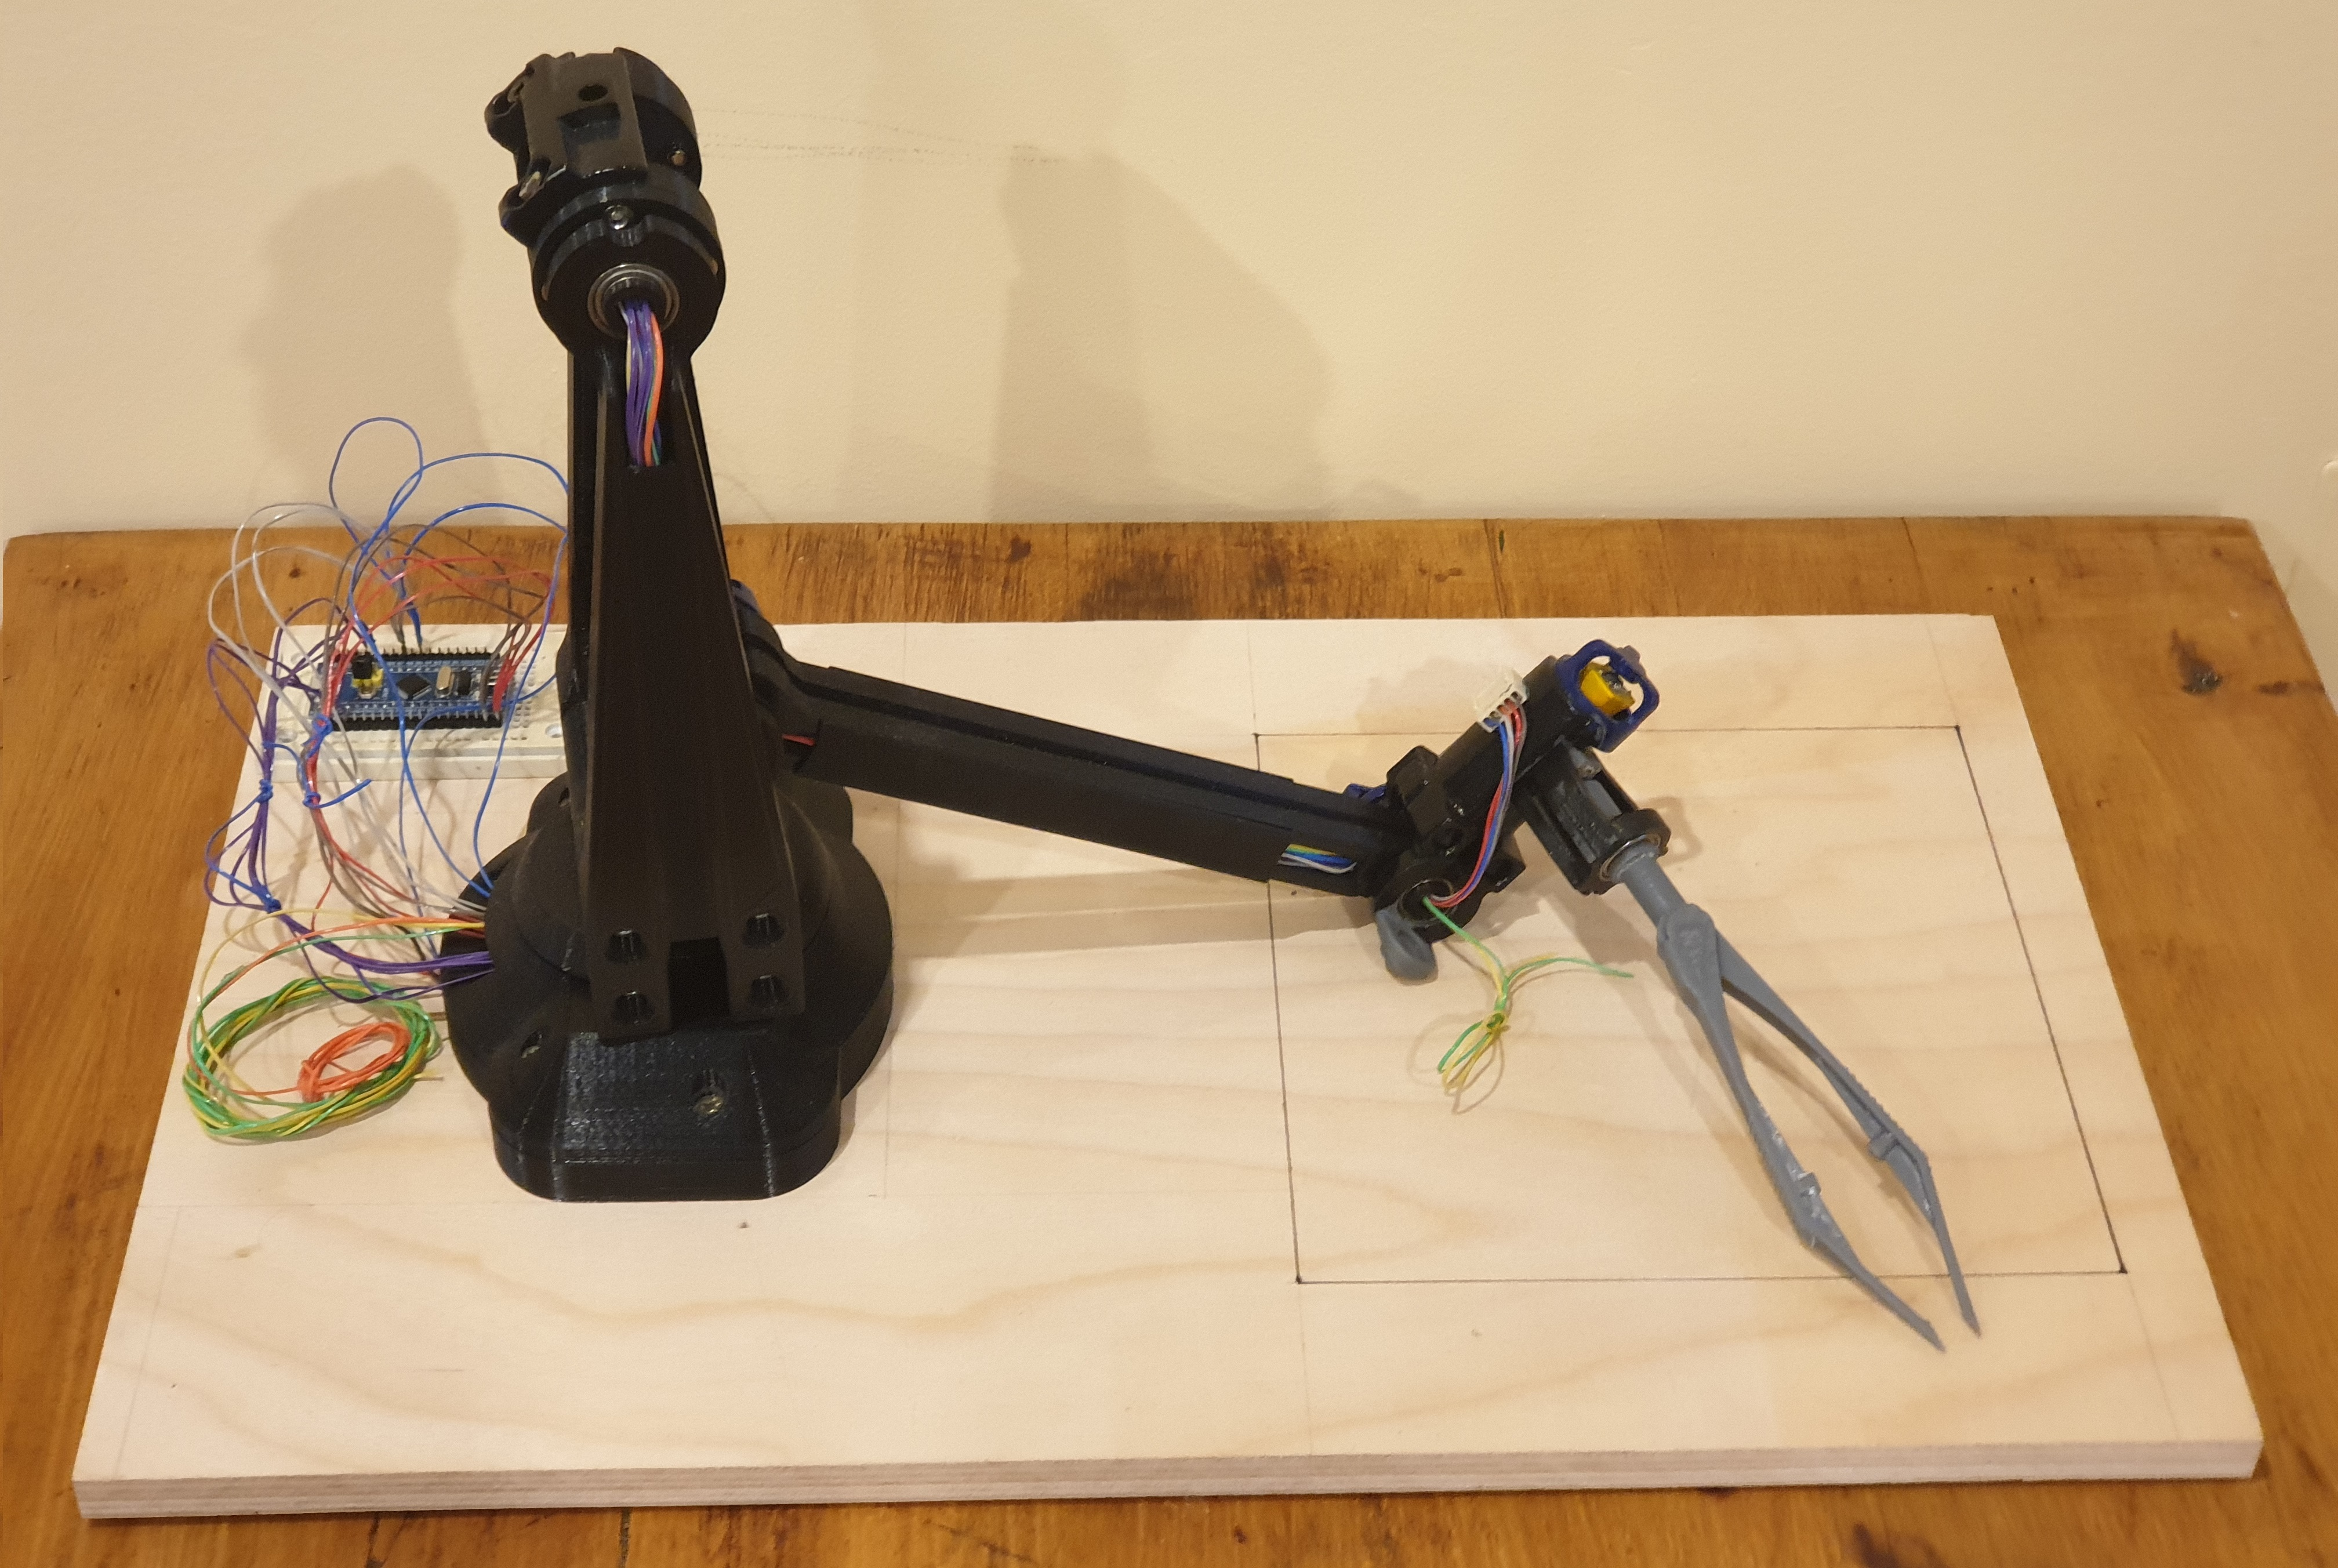
\includegraphics[width=150mm, keepaspectratio]{figures/Szakdoga/0_v_4_csipeszes}
\caption{Szakdolgozatomban elkészített telemanipuláto}
\label{fig:Szakdoga_csipeszes}
\end{figure}

Nagyon fontosnak tartottam, hogy a megtervezett eszközt el is készítsem valamilyen formában, mivel így sokkal alaposabban megtudtam vizsgálni az eszközt. A telemanipulátor 3D nyomtatással lett elkészítve. A FDM\footnote{Fused Deposition Modeling - A nyomtatási technológia a hőre lágyuló polimerekkel képes 3D-s objektumokat nyomtatni. Az FDM nyomtatók azzal az alapelvvel működnek, hogy szobahőmérsékleten szilárd hőre lágyuló polimert 180$^{\circ}$- 300$^{\circ}$C-ra melegítve ömledéket állapotba kerülnek és a kívánt helyre lehet juttatni lineáris vezetékrendszer segítségével.} technológiával készült, viszont néhány alkatrész, mint például a szenzortartó elkészítéséhez SLA\footnote{StereoLithography Apparatus - modellteret UV aktív gyantával tölti fel. A nyomtatási térben egy síklapra építi fel a tárgyat úgyhogy, az belemerül egy gyantával teli kádba, ahol a megfelelő rétegvastagságú folyékony gyanta réteget UV lézerrel térhálósítja és köti adhézióval az előző réteghez} módon működő nyomtatót használtam. 

 % 2. fejezet
\chapter{Telemanipulátor geometria tervezése}
\label{sec:LatexTools}

Az általam tervezett telemanipulátor egyesíti mindazt, amit a teljes képzés során elsajátítottam. 

%----------------------------------------------------------------------------
\section{Korábbi eszközzel kapcsolatban levont következtetések}
%----------------------------------------------------------------------------
\section{Újratervezési szempontok}
%----------------------------------------------------------------------------
\section{Geometria kialakítása}
%----------------------------------------------------------------------------      % 3. fejezet
\chapter{Telemanipulátor jelfeldolgozó rendszere}
\label{sec:elektronika}

A bemutatott fizikai rendszerhez tartozó jelfeldolgozó rendszer hardveres elemei nem sokban térnek el a szakdolgozatomban használt megoldásoktól. Mégis jelentősen összetettebbé vált az elmúlt két évben azáltal, hogy mennyi mindent sajátítottam el a képzés végére. Kiegészítettem néhány biztonsági és jelminőséget javító funkcióval. Ebben a fejezetben igyekszem részletesen bemutatni a telemanipulátor aktuális pozíciójának meghatározására kiválasztott szenzorokat és a mikrovezérlőt.

%----------------------------------------------------------------------------
\section{Jelfeldolgozó rendszer koncepciója}

A komponensek bemutatása előtt a szögmérésre felépített rendszer elvét szeretném bemutatni. A rendszernek hasonlóan a fizikai vázhoz a tervezés során meghatározott elvárásoknak kell megfelelnie. Ugyan a \ref{sec:ujratervezesi_szempontok} fejezetben felsorolt elvárások száma lényegesen kisebb mint a vázzal vagy a programmal szemben támasztottak, viszont legalább annyira lényegesek. Komolyabb teljesítmény elektronikát nem kellett tervezzek a rendszerhez, mert a kiválasztott mikrovezérlő DC kimenete bőven képes előállítani a szenzorok feltáplálásához szükséges áramot. Amit viszont már a fizikai rendszer tervezésénél figyelembe kellett vennem, hogy a kábelezés ne legyen túl nehézkes, hogy a kommunikációban a szenzor-mikrovezérlő távolságból származó ellenállás ne okozzon problémát. A szenzorok tesztelésénél foglalkoztam a maximálisan használható drót hossz megállapításával. A rendszert a lehető legegyszerűbben, a lehető legkevesebb egyedi alkatrész felhasználásával készítettem el. A hangsúlyt a \ref{sec:mikrovez_bemut}.fejezetben bemutatásra kerülő mikrovezérlő kiválasztására fektettem. Nem volt szükség méret vagy egy fizikai korlát használatára, így igyekeztem a lehető legnagyobb teljesítményű és legtöbb potenciális továbbfejlesztést lehetővé tévő megoldást választani. A következőkben a már megépített rendszert és a lehetséges továbbfejlesztési lehetőségeket bemutatni.

\begin{figure}[!ht]
\centering
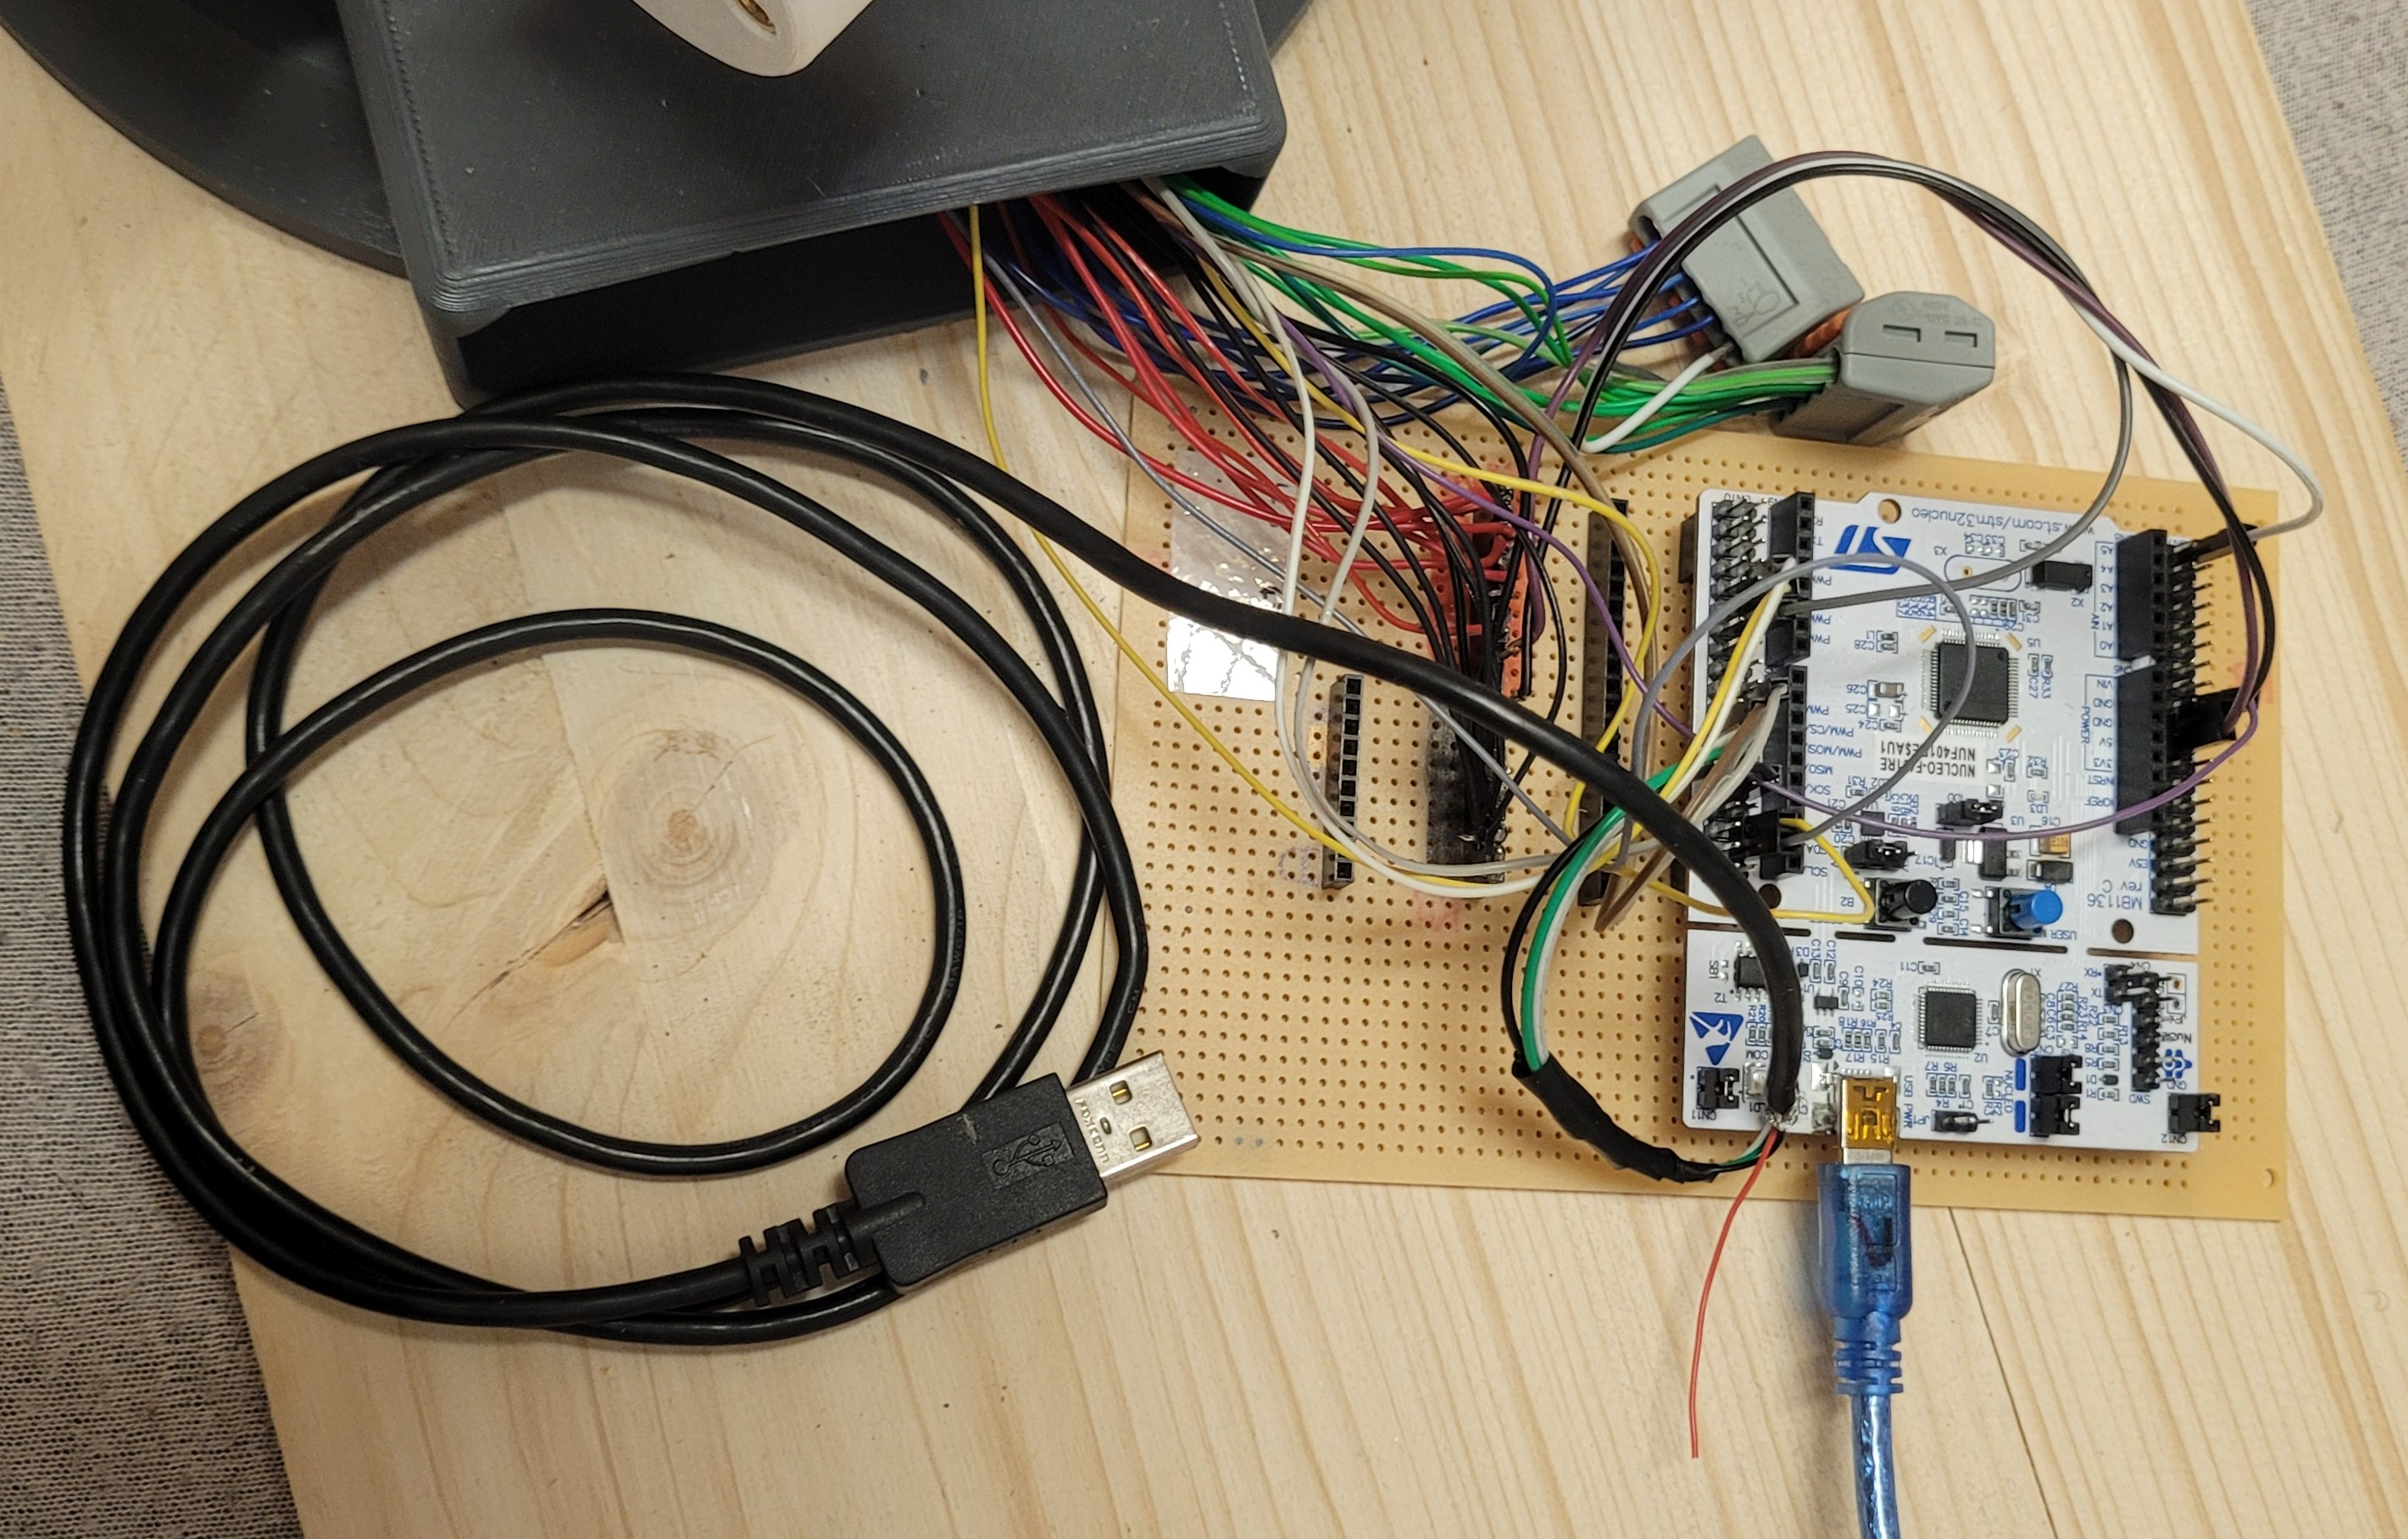
\includegraphics[width=100mm, keepaspectratio]{figures/Csuklo_szog_teszt/mikrovez_2}
\caption{Az elkészült jelfeldolgozó rendszer}
\label{fig:mikrovez_2}
\end{figure}

%----------------------------------------------------------------------------
\section{Jelfeldolgozó rendszer összeállítása}

A jelfeldolgozó rendszer elektronikai oldalról minimális mérnöki ismeretekkel is könnyen megérhető és a bemutatása is igen egyszerű. Az összeállítást a csuklóban érzékelt szögtől indulva mutatom be lépésről-lépésre. Egy adott csuklóból induló két kar egymással bezárt szögének mérésére GMR(Giant magnetoresistance) szenzort használtam. A szenzor működését \ref{sec:gmr_leiras}.fejezetben részletesen bemutatom. A szenzor összeállítás magából a szenzorból és a szenzorlapjával párhuzamba állított mágnesből áll. Ezzel a szenzor összeállítással a jeladó és a jelvevő között fizikai kontaktus nélkül tudok szöget mérni. Viszont ami még lényegesebb nincs végállása a szenzornak. Így a váz tervezése során csak azt kellett figyelembe vennem, hogy a szenzor és a mágnes középtengelye egybe essen és a távolságuk ne legyen nagyobb mint $17[mm]$. A szenzorhoz saját magam által tervezett és gyártott NyÁK lapot használtam, mivel a szenzor SMD\footnote{ Surface Mount Device rövidítése, magyarul felszíni szerelésű eszköz. Az SMD elektronikai elemek olyan alkatrészek, amelyek kis méretűek és a nyomtatott áramköri lap felszínére vannak forrasztva.} kivitelű, ezért szükséges volt megoldani a szenzor chip lábai és a drót közötti kapcsolatot.

\begin{figure}[!ht]
\centering
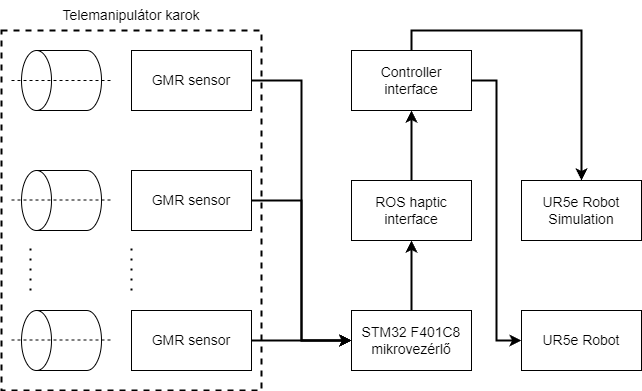
\includegraphics[width=125mm, keepaspectratio]{figures/Diagrammok/Telemanipulator_teljesrendszer}
\caption{A jelfeldolgozó rendszert szemléltető ábra}
\label{fig:Telemanipulator_teljesrendszer}
\end{figure}

A következő fontos komponens a bypass kondenzátor. Ennek a kondenzátornak a célja a teljesítmény ingadozás kiküszöbölése, ezzel a szenzor működése egyenletesebbé tehető. Ezt a javaslatot a bypass kondenzátor használatára még a szakdolgozatom bírálatánál kaptam, mint lehetséges teljesítmény javító komponens.

Tovább folytatva a bemutatást, részletesebben szeretném bemutatni a drótok csatlakozóit, ugyanis a szakdolgozatban elkészített telemanipulátor szenzoraihoz tartozó drótok nem voltak megbonthatóak az összeállítás teljes hosszában. Ez a későbbi továbbfejlesztési lehetőséget akadályozta meg. Ebben a dolgozatban bemutatott eszköznél már a váz fizikai paramétereinek megadásánál figyeltem, hogy csatlakozókat tudjak a szenzoroknál elhelyezni. A végső változatban a szenzor után $30-40[mm]$-re helyeztem el minden bontó csatlakozót, hogy a tengelyeket a mozgásban ne akadályozza, de bármilyen probléma esetén könnyen hozzáférhető legyen. Ez az extra elem a későbbiekben a leghasznosabb fejlesztésnek bizonyult, ugyanis a szenzorok üzembe helyezése alatt a hiba keresést leegyszerűsítette, hogy nem kellett a mikrovezérlő bekötéseit megbontanom ahhoz, hogy külön leellenőrizhessem a működést.

A megfelelő drót kiválasztás a nem kritikus, de érdemes odafigyelni. Két hardver szempontjából lényeges kritériumot fogalmaztam meg és két szerelési kritériumot támasztottam ezzel szemben. Ezek a következőek voltak:

\begin{itemize}
  \item A drótnak a minimális fordulási sugarának alacsonynak kell lennie. Ez azért fontos, mert a szakdolgozatnál készített manipulátor esetében ezt nem vettem figyelembe és a drótok a használat közbeni deformációja nehezítették a mozgatást
  \item A drót egységnyi hosszon mért ellenállása ne akadályozza a szenzorok működését. Ez kevésbé fenyegető probléma, azonban érdemesnek tartottam figyelembe venni, ugyanis a hatodik szenzor és a mikrovezérlő távolsága megközelíti $1000[mm]$-t. Ez a későbbiekben bekövetkező tovább fejlesztést akadályozhatja meg.
  \item Szerelési kritériumként figyelembe vettem a drótok maximális átmérőjét. Több esetben 2-3 szenzorhoz tartozó kábelezés lép át egy adott csuklóban egyik karban futó csatornából a másikba. A probléma leküzdését két oldalról közelítettem meg. Egyrészt a maximális drót számhoz tartozó átmérőnek a $400[\%]$-át vettem minimum keresztmetszetnek minden csuklóban. Másodsorban szignifikánsan nagyobb csapágyakat választottam mint a szakdolgozatomban, így gyakorlatilag akár 20-30 szenzor elvezetése is lehetséges lenne a csukló tengelyeknél.
  \item A szerelés megkönnyítésére nagyon fontos és az egyszerű hibakeresésnél lényeges, hogy minden szenzorhoz tartozó a szenzorválasztójelét továbbító drót jól megkülönböztethető legyen. Röviden megfogalmazva a drótból, amit választok legalább $11$ féle szín legyen elérhető. Ez a gond a szakdolgozatban épített telemanipulátor újra indításánál jelentkezett. Rengeteg időt vett el a szenzorok újra beazonosítása.
\end{itemize}

Ezek a meghatározott kritériumok egy része kényelmi és inkább magasabb bekerülési költséget eredményeznek, de a teljes rendszer finanszírozhatóságával később szeretnék foglalkozni.

A következő komponensek már lényegesen összetettebbek. Logikai sorrendben a mikrovezérlő(MCU\footnote{Micro Controller Unit - magyarul mikrovezérlő}) következik. Az MCU végzi a szenzorok áramellátását, velük való kommunikációt, az adatok feldolgozását és ezek továbbítását. Az MCU program leírását a \ref{sec:MCU_program}.fejezetben részletesebben is megteszem. A mikrovezérlő USB kommunikációs porton csatlakozik a számítógépre, míg a saját bootloaderével\footnote{A bootloader egy speciális szoftver, amely lehetővé teszi az alkalmazásfirmware frissítését vagy telepítését a mikrovezérlőn keresztül.} a program felügyeletét lehet végezni.

%----------------------------------------------------------------------------
\section{Elektronikai rendszer komponensei}

A komponensek kiválasztása egyes esetekben más és más szempontok alapján történik. Az egyik oka, hogy költségelemezést végeztem a telemanipulátorral kapcsolatban a dolgozatom végén (XYZ fejezet), hogy egy átfogó képet készítsek arról, hogy jelenleg egy ilyen végletekig leegyszerűsített prototípus körülbelül mekkora előállítási költséggel jár. A komponensek kiválasztási szempontjaiban az elérhetőséget és a későbbi továbbfejleszthetőséget tartottam szem előtt. Az alkatrészek bemutatásánál nem térek ki a szerelvények minden elemére, mert például az USB kábel legoptimálisabb kiválasztására nem fektettem energiát. Csakúgy mint a rendszer koncepciós bemutatásánál szenzortól haladva a nagyobb egységekig fogom bemutatni az elemeket részletesebben.

%----------------------------------------------------------------------------
\subsubsection{GMR szenzor}
\label{sec:gmr_leiras}

A csukló szög megállapításához használt szenzor összeállításban a korongmágnes állását mértem egy mágneses térorientációt mérni képes szenzorral. A Giant Magnetoresistance (GMR) egy olyan érzékelő, amely az szenzorban található ellenállások elektromágneses tulajdonságaiknak változását méri egy mágneses mező hatására. Ez a technológia a mágneses rezisztivitás változását használja ki, amikor egy mágneses tér hatására az elemben levő részecskék mágneses állapota változik. A szenzor működése röviden úgy foglalható össze, hogy a szenzorok több réteg vékony filmrétegből állnak, amelyek között ferromágneses és nem-ferromágneses rétegek váltakoznak. A ferromágneses rétegek mágneses polarizációjukat megváltoztathatják a külső mágneses tér hatására, és ezáltal befolyásolják az elektromos ellenállást az érzékelőben. Ennek a változásnak a szenzorba mérőrendszer képes a mágneses pólusok orientációját megadni a szenzor tengelyeihez képest.

\begin{figure}[!ht]
\centering
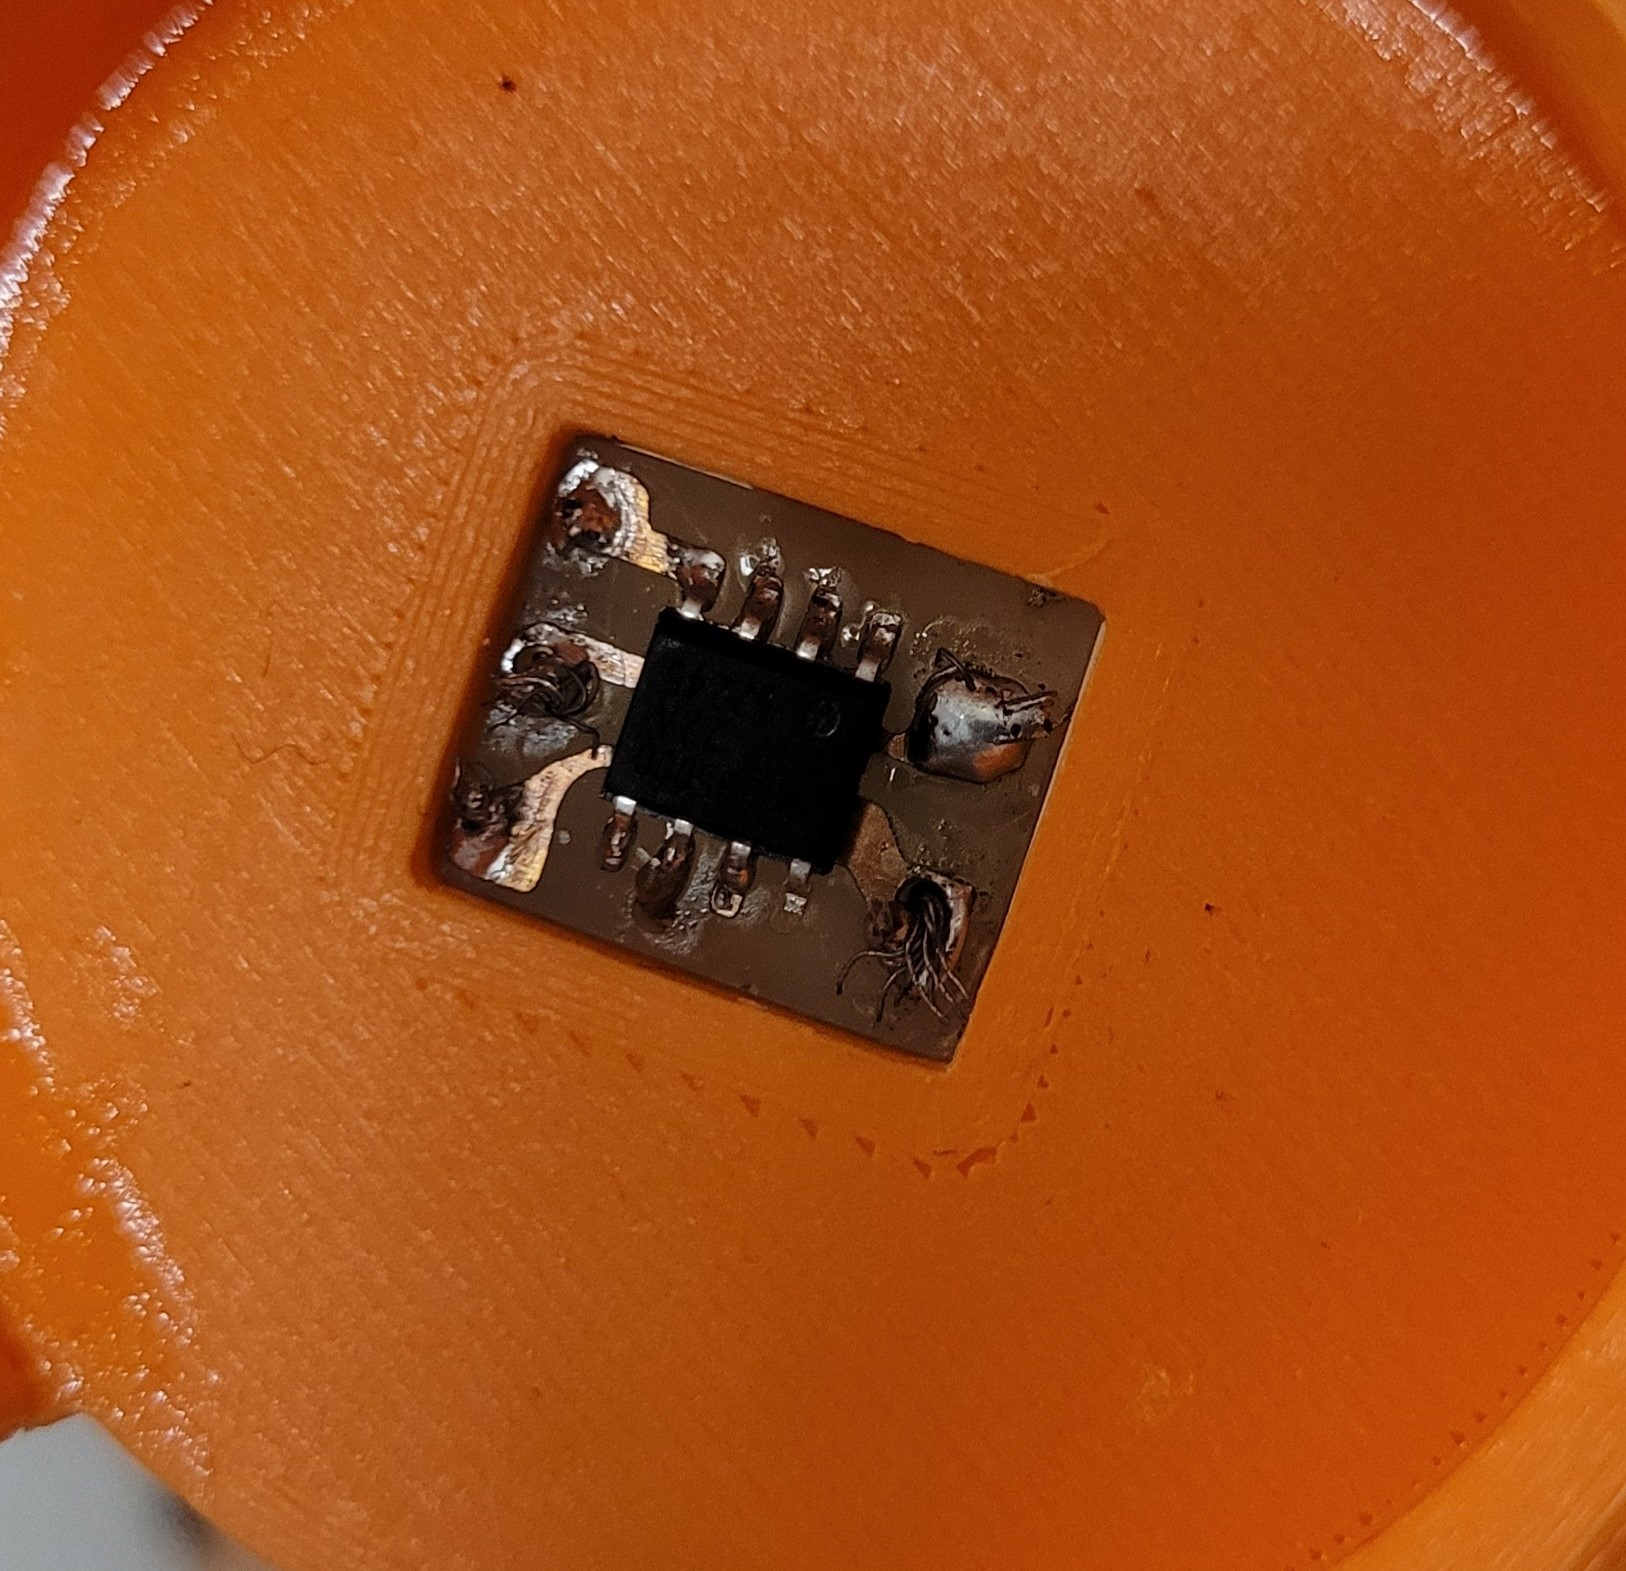
\includegraphics[width=65mm, keepaspectratio]{figures/Csuklo_szog_teszt/szenzor}
\caption{A NyÁK lapra helyezett GMR szenzor}
\label{fig:csuklo_szenzor_pcb}
\end{figure}

Az általam használt szenzor az Infineon TLE5012B jelzésű GMR szenzor. Ez a szenzor egy $360[^\circ]$-os szögérzékelő. Ezt az érzékelést monolitikusan integrált\footnote{A monolitikus integrált áramkörben az áramkör valamennyi aktív és passzív elemét, valamint a hozzájuk tartozó összekötéseket egyetlen chip-ben alakítják ki. Ezt a kialakítást szokás félvezető alapú integrált áramkörnek is nevezni.} Giant Magneto Resistance (GMR) elemekkel mérik, melyek a szinusz és koszinusz szögkomponenseit érzékelik a mágneses pólusoknak. Ezeket a nyers jeleket belsőleg digitálisan feldolgozzák a mágneses tér orientációjának kiszámításához. Ami nagyon fontos, hogy ez az érzékelő egy előre-kalibrált érzékelő. A kalibrációs paramétereket belsőleg tárolják. A bekapcsoláskor ezekhez viszonyítva adja meg a szögértékeket a szenzor. A szögmérés pontosságát egy opcionális belső automatikus kalibrációs algoritmussal lehet javítani a hőmérséklettartomány  és élettartam függvényében. Én ezt a funkciót nem használtam, de a mikrovezérlő programjába integráltam ennek a lehetőségét, de erről majd a \ref{sec:Prog_nagy_fej}.fejezetben a szenzor programozása kapcsán említést teszek. Az adatkommunikációt egy kétirányú Szinkron Soros Kommunikációval\footnote{A \ref{sec:ssc_kom}.fejezetben részletesen bemuatatom} (SSC) valósítják meg, amely SPI-kompatibilis. Utóbbi azért fontos, mert legelterjedtebben a SPI protokoll elérhető a mikrovezérlőknél. A szenzor konfigurációja regiszterekben tárolódik, amelyek elérhetők az SSC interfésszel. Emellett négy másik interfész is rendelkezésre áll a TLE5012B-vel: Impulzus-Szélesség-Moduláció (PWM) Protokoll, Rövid PWM Kód (SPC) Protokoll, Hall Kapcsoló Mód (HSM) és Inkrementális Interfész (IIF). Ezeket az interfészeket az SSC-vel együtt vagy önállóan lehet használni. Előre konfigurált érzékelő változatok elérhetők különböző interfészbeállításokkal, de a telemanipulátornál én, csak a SSC kommunikációs megvalósítást használtam. Ez a legegyszerűbb és az általam használt program könyvtár is erre volt optimalizálva. Néhány fontosabb jellemzőt még felsorolok a szenzorról, amik fontosabbak:

\begin{itemize}
	\item Egy chipben van minden. Nincs szükség további komponensre a szenzor működtetéséhez.( A bypass kondenzátor is inkább csak pontosság és megbízhatóság javító kiegészítő )
	\item $360[^\circ]$-os szögmérés fordulatszámlálóval és szögsebesség méréssel. Ugyan nem használom ki szögsebesség mérést, de mint lehetőség későbbiekben a gravitációs hatásából származó terhelés kikompenzálásában még szerepe lehet. A $360[^\circ]$-os mérés pedig külön előny, hogy nem kell foglalkozni az összeszerelésnél az orientációval, offszeteléssel be lehet könnyedén állítani.
	\item 15 bites szögérték megadás a kimeneten, aminek pontossága $0,01[^\circ]$. Ez kellően nagy felbontás ahhoz, hogy a telemanipulátor end-effektorának pozícióját meghatározzam
	\item 16 bit-en értelmezett szinusz / coszinusz érték az interfészen
	\item Maximum $1[^\circ]$ hiba a gyártó által garantálva, szenzor élettartalma és környezeti hőmérséklet függvényében
	\item Két irányú SSC kommunikációs protokol az interfészen, ami $8[\frac{Mbit}{s}]$-ig emelhető. A szenzor mérés szögmérésének periódus ideje minim $0,001366[ms]$, ami bőven a $4[ms]$-os cél érték alatt van.
	\item Számos egyéb kommunikációs protokoll \textbf{SSC}, PWM, IIF, HSM, SPC
	\item A chip választó pin többféleképpen konfigurálható. (push-pull vagy open-drain)
 	\item Magas hőmérséklet tűréshatár: $-40[^\circ C]-tól~150[^\circ C]-ig$
	\item Nem tartalmaz halogént
\end{itemize}

\begin{figure}[!ht]
\centering
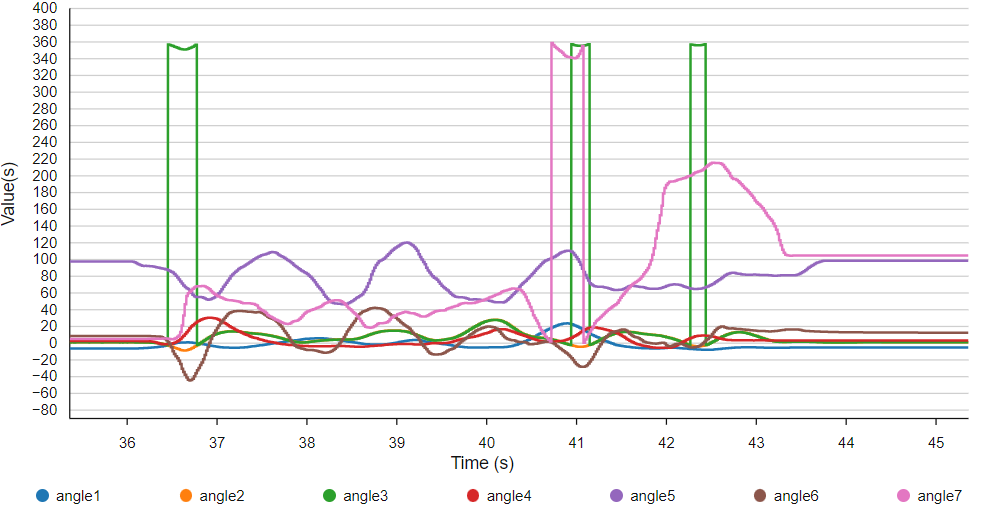
\includegraphics[width=100mm, keepaspectratio]{figures/Csuklo_szog_teszt/szumma}
\caption{Az csuklóban található szenzorok működés közben}
\label{fig:csuklo_teszt_szumma}
\end{figure}

Ez a szenzor kellő megbízhatóságú a tapasztalataim alapján, kézi forrasztás közben jól kezelhető és nem érzékeny a magas forrasztási hőmérsékletre. Kifejezetten pontos és rendkívül gyors számítással rendelkezik ezért ideális a telemanipulátorhoz tartozó karok szögértékének mérésére. A dolgozatomban még kitérek a szenzorok tesztelésére.

%----------------------------------------------------------------------------
\subsection{Bypass kondenzátor}

A szakdolgozatom bírálásában kaptam javaslatként, hogy egészítsem ki a szenzor NyÁK-ot egy bypass kondenzátorral. A képzésem további szakaszában részletesebben tanultunk is erről a típusú alkalmazási lehetőségről a kondenzátorok esetében. A bypass kondenzátorok olyan elektromos komponensek, amelyeket általában abból a célból alkalmaznak, hogy a stabilitást, zajszűrést és teljesítményjavulást érjenek el. Ezek a kondenzátorok képesek "bypass"-olni, azaz át vagy elvezetni az áramot bizonyos alkatrészek mellett. Kicsit részletesebben bemutatnám a kondenzátor működését és azt, hogy mely jellemzőket kihasználva lehet ezt a bypassoló hatást elérni. A kondenzátorok alapvetően két vezető lemez között elhelyezkedő dielektromos anyagból állnak. Amikor az elektromos feszültség megváltozik, a kondenzátorban tárolt elektromos töltés is változik. Ennek eredményeként a kondenzátor karakterisztika függvényében felhalmozza majd átengedi az áramot. Ha ez periodikusan megtörténik, akkor a kondenzátor bizonyos frekvenciákon, akár a zajt vagy pusztán teljesítmény stabilitást adhat a rendszernek. Utóbbi jelenséget használjuk ki bypass kondenzátor esetében. Ezt a kondenzátor használati módot gyakran alkalmaznak a következőkbe felsorolt esetekben:

\begin{itemize}
	\item Zajszűrésre, különösen érzékeny elektronikai eszközök, például erősítők vagy analóg- digitális átalakítók környezetében. Ezek a kondenzátorok képesek alacsony frekvenciájú zajokat szűrni, javítva ezzel a jelerősséget.
	\item Stabilitás javítására, például mikroprocesszorok vagy más integrált áramkörök esetében a kondenzátorok segítenek kiegyenlíteni a feszültség-ingadozásokat.
\end{itemize}


\begin{figure}[!ht]
\centering
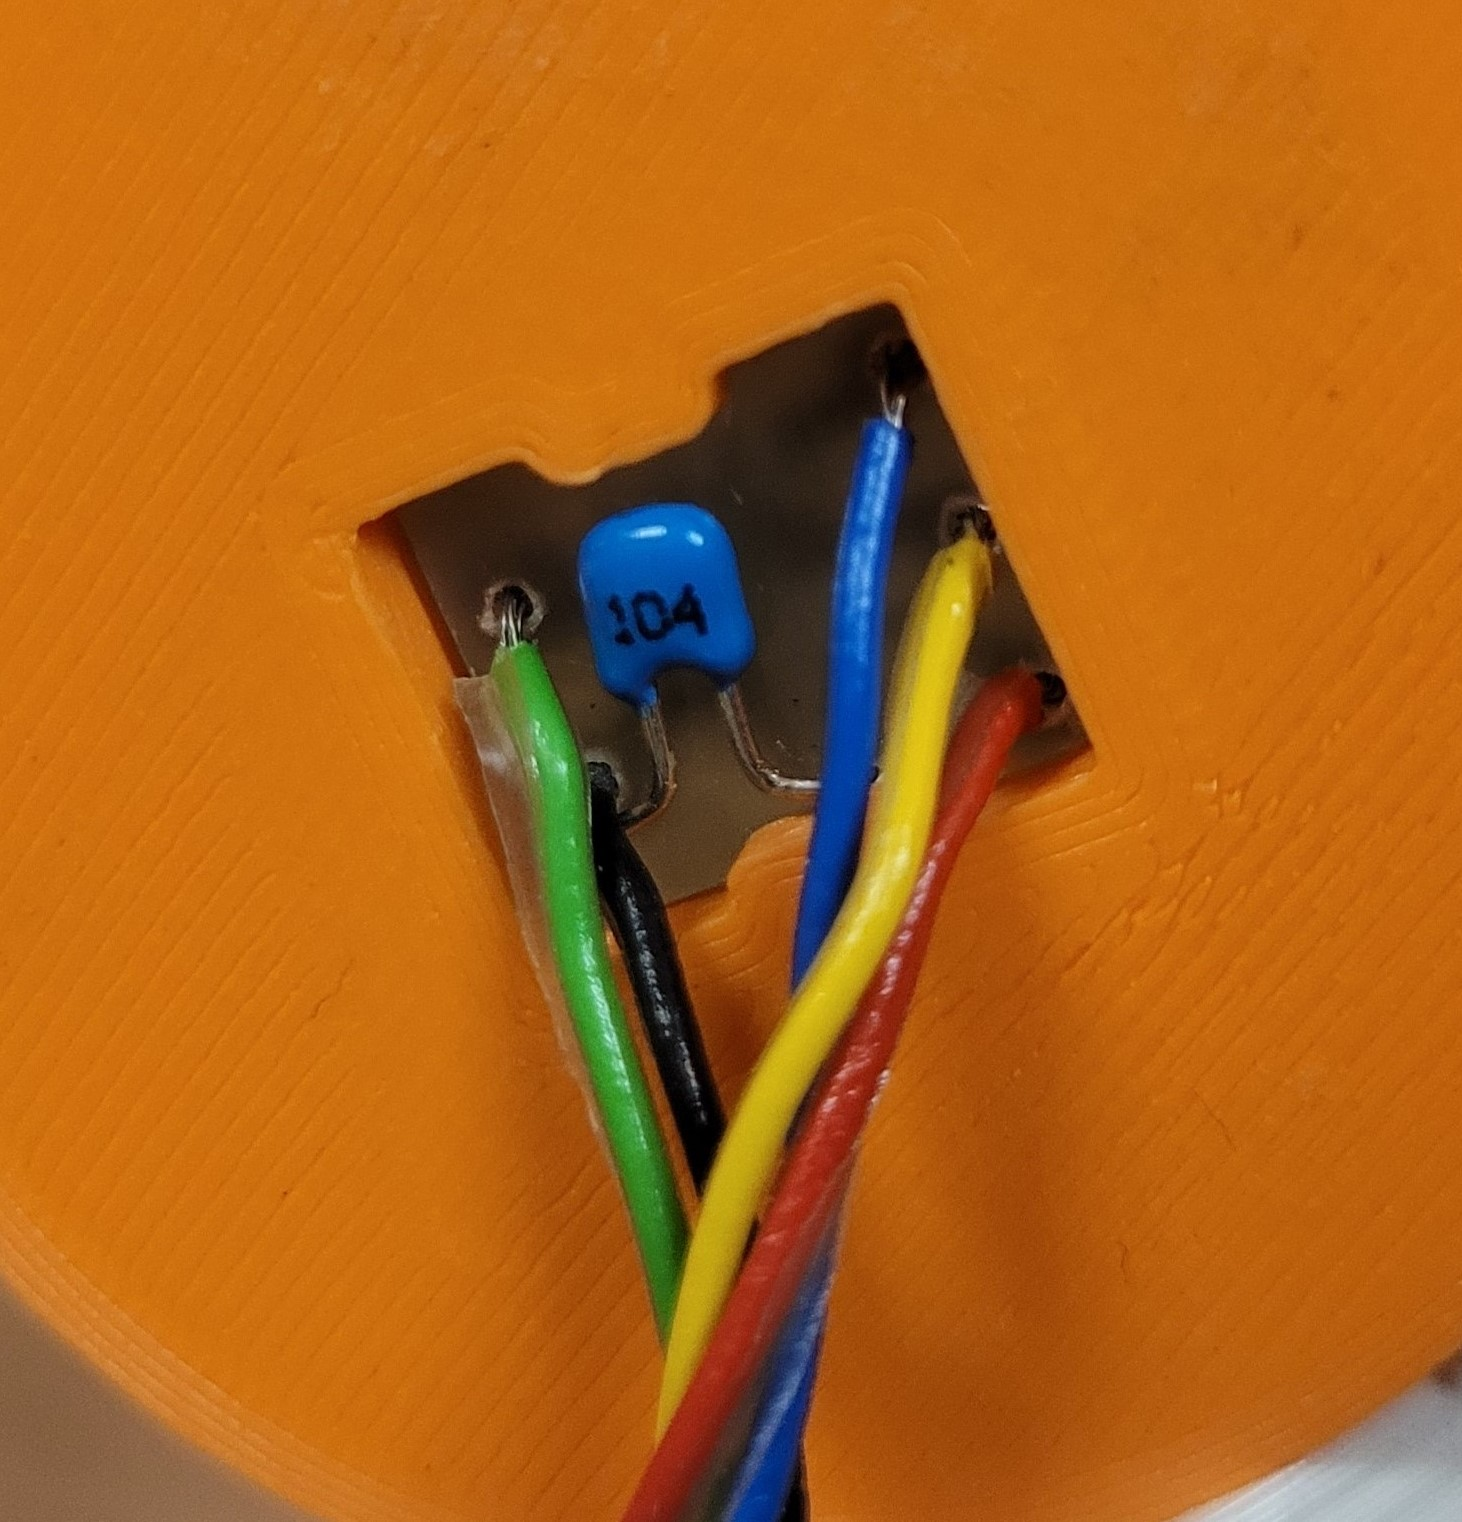
\includegraphics[width=70mm, keepaspectratio]{figures/Csuklo_szog_teszt/bypass}
\caption{A szenzoron található bypass kondenzátor beépítve}
\label{fig:bypass}
\end{figure}

A bypass kondenzátor elhelyezése kritikus a hatékony zajszűrés és kellő stabilitás szempontjából. A kondenzátort a szenzort tápláló lábak közvetlen közelébe kell elhelyezni. A képen is jól látható módon én a szenzor $3V3$-as lábának helye mellett helyeztem el a furatot, ennél közelebb nem-igen tudtam volna fúrni rögzítőfuratot. A $GND$ azaz föld a kondenzátor másik lába esetében annyira már nem fontos.

A megfelelő bypass kondenzátor kiválasztása fontos a kívánt teljesítmény eléréséhez. A kondenzátor értéke és típusa is nagymértékben befolyásolja a hatékonyságot. Az általam választott kondenzátor $100[nF]$-os $50-[V]$-os nyitó feszültséggel rendelkező kerámia kondenzátor. Az ilyen típusú kondenzátorok kiválóan teljesítenek magas frekvenciás alkalmazásokban, amelyekhez gyakran használják őket bypass kondenzátorként. Rendkívül jól használhatóak stabilitás és zajszűrés céljából. Kis méretűek és alacsony induktanciájúak, ami különösen fontos, mivel a szenzor kompakt és nem igen kiegészíthető más elemmel a zavaró jelek kiszűrése érdekében. Ezek mellett a kerámia kondenzátorok elérhetők különböző kapacitásértékekkel míg a méretük meglehetősen kicsi, így jól használhatóak kis méretű szenzorok esetében is, amilyenre nekem is szükségem van. A későbbiekben is ki fogok rá térni, de ezek a kondenzátorok általában gazdaságosak, ez hozzájárul a bekerülési költségek csökkentéséhez.

A kondenzátornak a paraméterei bőven túlméretezettek\footnote{Ennek a nyitó feszültség értéknek a fele is elegendő lenne a rendszer stabilitásának biztosítása érdekében}, mérete kellőképpen kicsi, olcsó és majdnem minden kiskereskedelmi egységben beszerezhető.

%----------------------------------------------------------------------------
\subsection{Csatlakozók}

Korábban említettem és a kritériumok közt is szerepelt, hogy minél flexibilisebbre szerettem volna a rendszert megtervezni. Ennek céljából külön odafigyeltem a csatlakozókra, hogy milyet használjak. A legkézenfekvőbbnek a MOLEX gyártó által elérhető csatlakozók bizonyultak. Ezek széles körben használt elektromos csatlakozók, és számos előnyt kínálnak, amelyek miatt népszerűek az elektronikai és ipari alkalmazásokban. Legnagyobb előnye, hogy a csatlakozók moduláris kialakításúak, ami lehetővé teszi, hogy kialakíthassunk velük egyszerű vagy összetett csatlakozási rendszereket az adott alkalmazáshoz. Ez a típus gyorsan és könnyen csatlakoztatható és bontható. Ez gyors telepítést és karbantartást tesz lehetővé, ami különösen előnyös összeszerelési, hibakeresési vagy fejlesztési esetekben. Széles körben alkalmazhatók különböző területeken, ennek eredményeként viszonylag egyszerű beszerezni. A Molex a minőségi termékeiről ismert, és csatlakozói megfelelnek a szigorú minőségi szabványoknak, ennek eredményeként a csatlakozók megbízhatóak és hosszú élettartamúak. Átfogó termékválasztékkal rendelkezik, beleértve különböző típusú csatlakozókat, vezetékeket, illetve kiegészítő termékeket. A telemanipulátor esetében 6 pin-es csatlakozókat választottam azért, hogy minden szenzornak saját vezeték párjai legyenek. Ezek a csatlakozók magas teljesítményű és nagy sebességű adatátvitelre alkalmasak, ami fontos volt a eszköz szempontjából. Ezeken felül a csatlakozók kis eséllyel kontaktosak\footnote{Rövid pillanatszerű vagy mozgásra vagy rezgésre megjelenő folytonosság hiba}, illetve az élettartalom se utolsó, mivel ezt a rendszer a lehető leggazdaságosabban a legtovább működteti.

\begin{figure}[!ht]
\centering
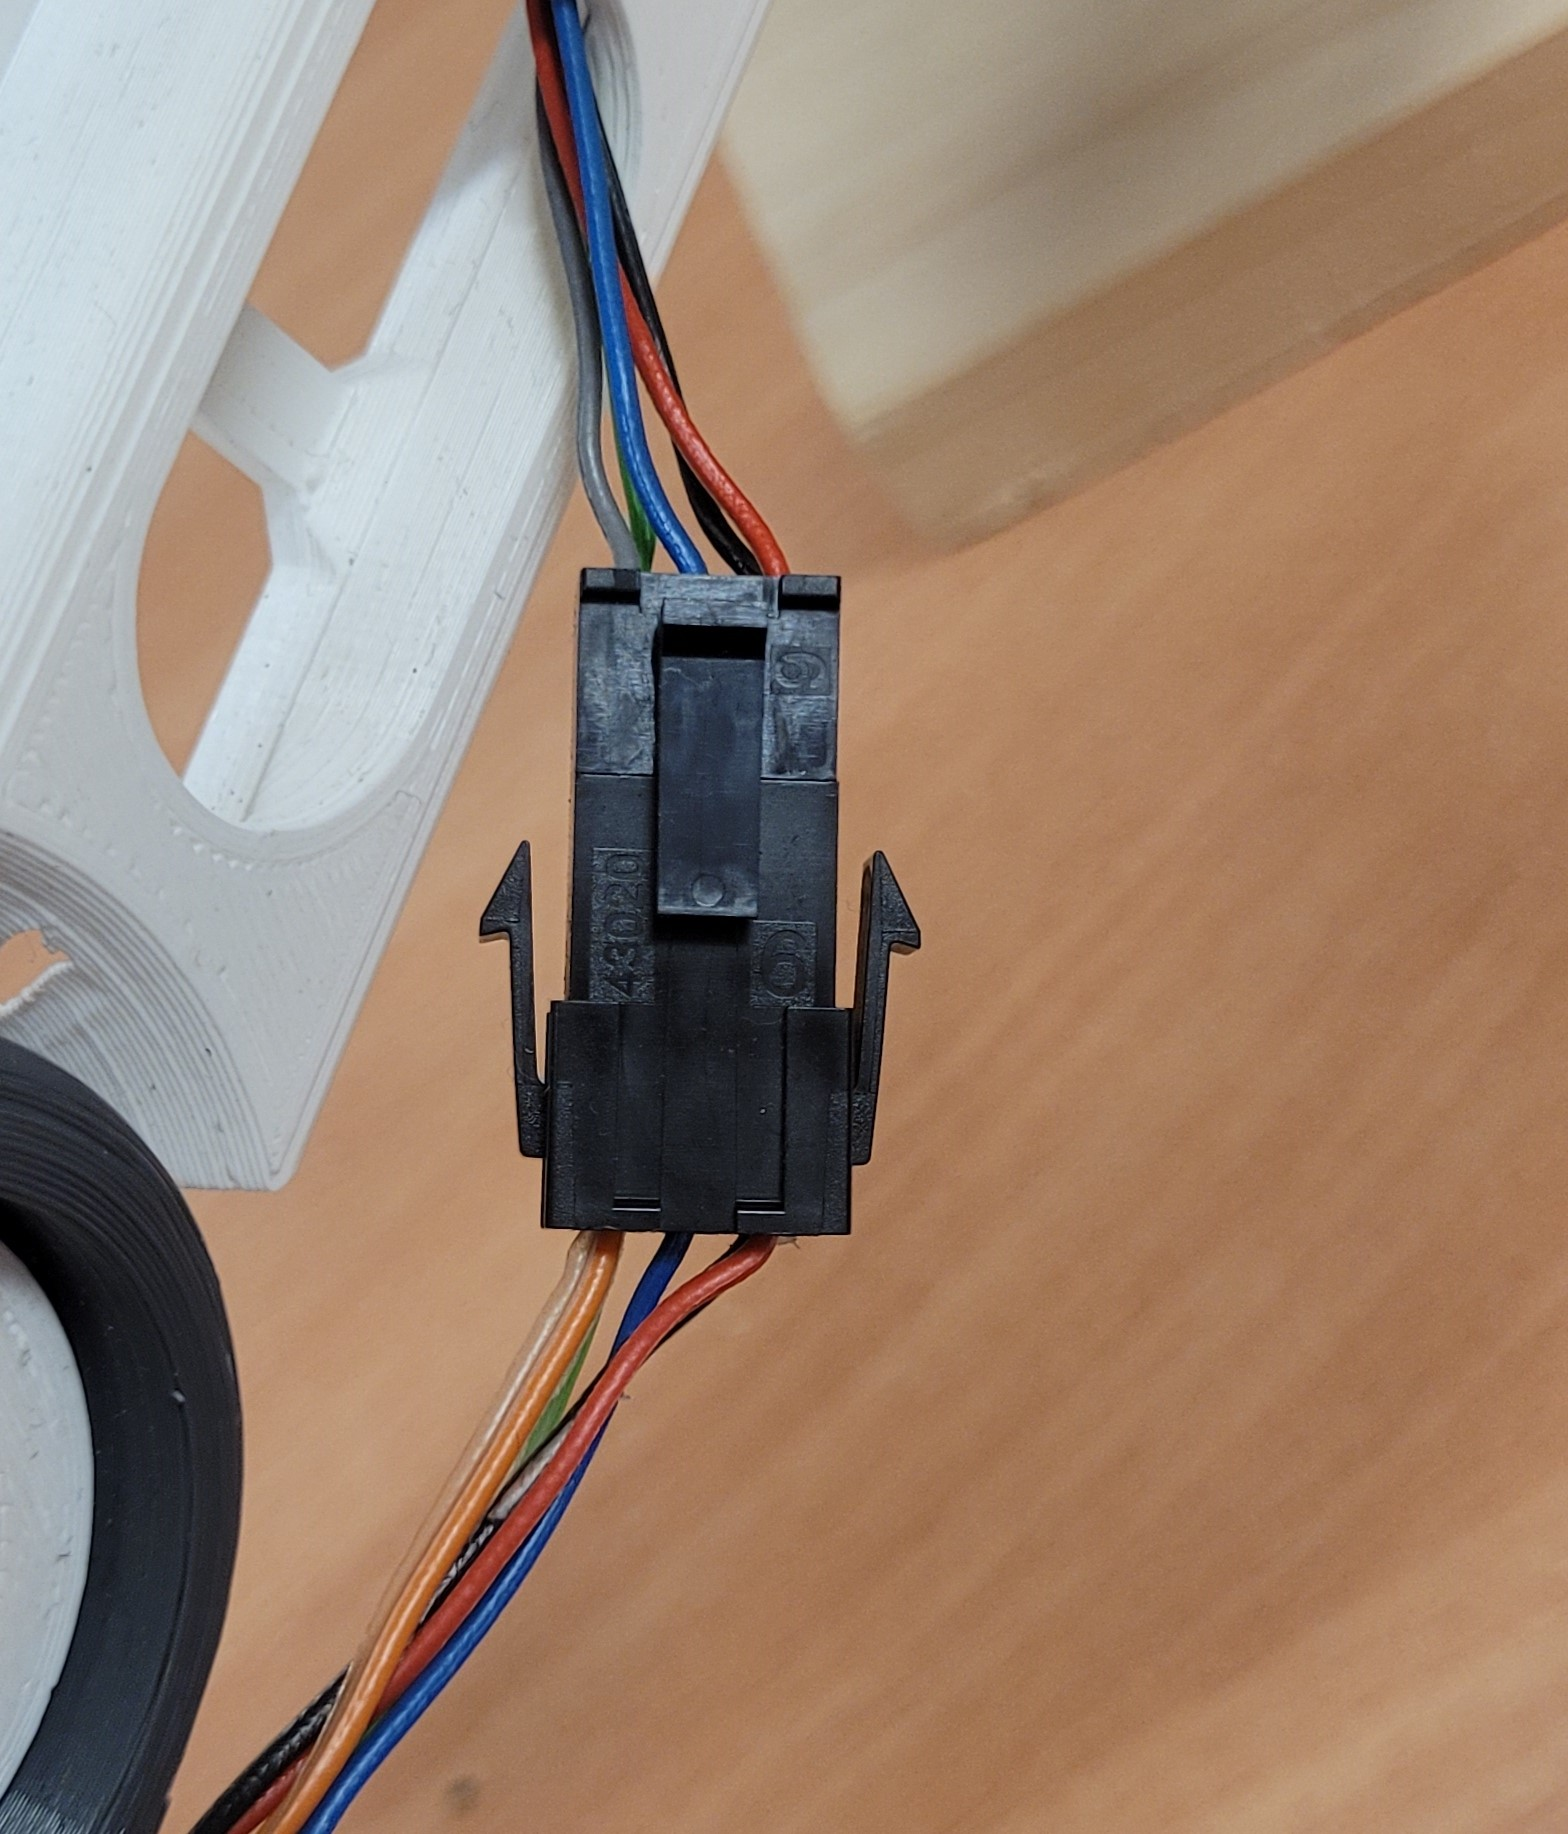
\includegraphics[width=60mm, keepaspectratio]{figures/Csuklo_szog_teszt/molex_valos}
\caption{A negyedik és ötödik kar között található szenzor csatlakozója}
\label{fig:csuklo_csatlakozo}
\end{figure}

\subsection{Mikrovezérlő}
\label{sec:mikrovez_bemut}

Elérkeztünk a mikrovezérlőig, mivel strukturálisan a vezetéken megérkező jeleket érzékelni tudjuk és a mikrovezérlőre csatlakoztatva az ezen futó programmal fel is tudjuk dolgozni. A szakdolgozatomban összeállított telemanipulátorhoz képest itt egy nagyobb komplexitású mikrovezérlőt választottam. Ennek az az oka, hogy a korábban használt eszközben nincs beépített bootloader, a pinek száma lényegesen kisebb és az eszköz memóriája túl kicsi a továbbfejlesztéshez. Ezek alapján döntöttem úgy, hogy a STMicroelectronics által gyártott Nucleo típusú fejlesztő board-ot választom. Az előnye a fejlesztő board-oknak, hogy a gyártó által összeállított tesztelt eszközök. Túlságosan nagy a felhasználhatóságuk, így könnyen pazarló vagy felesleges funkciókat is vásárolhatunk velük, de a prototípus gyártás elengedhetetlen elemei.

\begin{figure}[!ht]
\centering
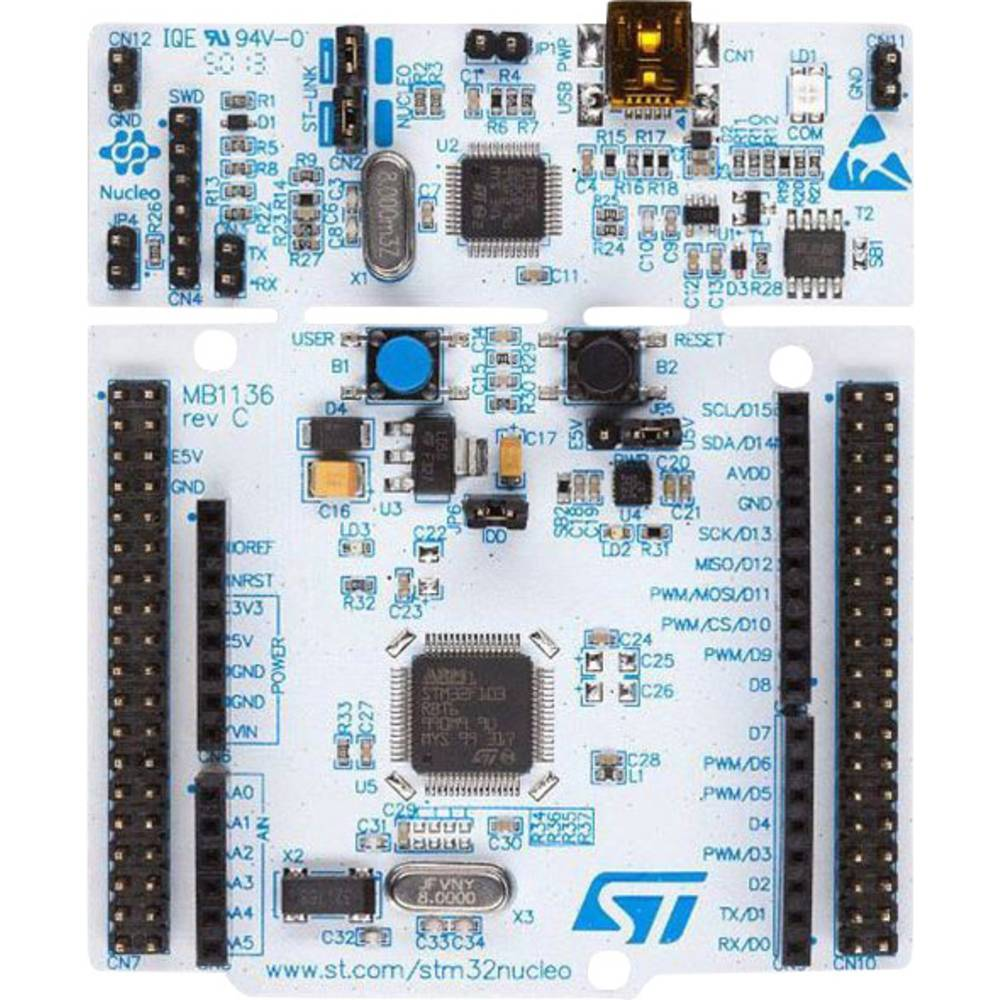
\includegraphics[width=60mm, keepaspectratio]{figures/Csuklo_szog_teszt/mikrovez}
\caption{Az csuklóban található szenzorok működés közben. A kép eredete: \url{https://www.st.com/en/evaluation-tools/nucleo-f401re.html}}
\label{fig:mikrovez}
\end{figure}

Az STM32 Nucleo boardok ezek alapján olyan fejlesztői platformok, amelyek kifejezetten az STMicroelectronics által gyártott STM32 mikroprocesszorokkal való alkalmazásfejlesztés támogatására szolgálnak. A board moduláris felépítésű, lehetővé téve a könnyű kibővítést és testreszabhatóságot. Érdekes előnyük, hogy a diákok körében elterjedt számtalan Arduino Uno és ST Morpho csatlakozók révén a felhasználók könnyen integrálhatnak kiegészítő modulokat, érzékelőket és egyéb hardvereszközöket az adott projekthez. Az STM32 Nucleo boardokat a STM32CubeIDE fejlesztői környezet támogatja, amely egyszerű és hatékony eszköztár a szoftverfejlesztéshez. Az STM32CubeMX grafikus konfigurációs eszköz segítségével könnyedén konfigurálhatók és beállíthatók a perifériák illetve a CubeMonitornak köszönhetően a grafikusan megjeleníthetőek a szenzor adatokhoz tartozó változók. Ennek az eszköznek nagy haszna volt amikor a szenzorok kalibrációját és tesztelését végeztem. A board beépített perifériákkal rendelkezik, mint például érzékelők, LED-ek és gombok, amelyek segítik a prototípusfejlesztést és a beágyazott rendszerek gyors tesztelését. Az én általam használt mikrovezérlő esetében $3[db]$ SPI (XYZ fejezet) kommunikációs port is található, amivel így a továbbfejlesztési lehetőségek száma nagyon megugrik. Az STM32 boardok nagyon jó minőségű és nagy terjedelmű dokumentációval rendelkeznek, beleértve az útmutatókat, példaprogramokat, fórumokat és alkalmazási jegyzeteket. Ennek a hasznosságát nem lehet kellőképpen nyomatékosítani, ugyanis pont a nagy terület lefedés miatt a boradoknál nagyon sok mindenre kell figyelni, hogy a lehető legjobb eredményt érjük el. Az utolsó általános szempont amivel a STM32 Nucleo boardaot vizsgálni lehet, hogy könnyen elérhetők a piacon, számos konfugurációban és a bekerülési költségük összevetve egy cél eszköz gyártásával is elég alacsony.

Az én általam használt STM32 Nucleo board pontos típusa STM32F401RE. A mikrovezérlő az egyik legújabb jelenleg és a háttértára kellő mértékben nagy ahhoz, hogy akár még kijelző vezérlésre is alkalmas legyen amellett, hogy a szenzorokat ugyanazzal a hatásfokkal kezelje, ami a $4[ms]$-os ciklusidő kritériumhoz kell. Az eszköz adatlapja elérhető a mellékletekben (\ref{sec:melleklet}.fejezet) és a részletes specifikáció ismertetése a \ref{sec:STM32_nucleo}, ezek mellett a előző eszközzel való összehasonlítására helyezném a hangsúlyt. A szakdolgozatom során egy STM32F103C8-as típusú mikrovezérlőt használtam. A könnyebb beazonosíthatóság érdekében a processzor típusa helyett a közismertebb nevét használom, ami a Bluepill.

A Bluepill típusú mikrovezérlő kompakt kisméretű, de tág fejlesztési határokat megengedő eszköz. Kis mérete, alacsony bekerülési költsége és alacsonyabb fogyasztása miatt használják. Jellemző felhasználási területe az IoT\footnote{Az Internet of Things az a koncepció, amely szerint különböző eszközök és egységek képesek kommunikálni az interneten, vagy felhőszolgáltatásokon keresztül. Jellemzően adatok gyűjtésére és megosztására használják. Illetve szoros összefüggésben van a "okos"/intelligens funkciók kialakításában.} (Internet of Things), kisebb autonóm rendszerek és adatgyűjtő berendezések. A diploma dolgozatomban bemutatott telemanipulátorhoz használt Nucleo-hoz képest, a Bluepill memóriája lényegesen kisebb, illetve a felhasználható perifériák száma is alacsonyabb. Azonban ez még nem tette szükségessé a lecserélését, inkább a jövőbeli fejlesztési lehetőségek számát korlátozná. A következő táblázatban összegyűjtöttem azt a néhány funkciót, ami miatt a mikrovezérlő cserére döntöttem.

\begin{table}[!h]
\begin{center}
    \begin{tabular}{|c c c|} 
        \hline
        Tulajdonság & STM32 F103C8 & STM32 F401RE  \\ 
        \hline
        Processzor típusa     &  Arm Cortex-M3  &  Arm Cortex-M4  \\
        Flashmemória          & $64[kB]$        & $512[kB]$       \\
        RAM mérete            & $20[kB]$    	& $96[kB]$        \\
        Beépített bootloader  & nincs           & van             \\
        SPI portok száma      & 2               & 3               \\
        \hline
    \end{tabular}
    \caption{STM32-es mikrovezérlő összehasonlítása}
\end{center}
\end{table}

A felsorolt különbségek száma nem sok, de a fejleszthetőséget nagy mértékben megkönnyíti. Az elkészült telemanipulátor jelfeldolgozó rendszer teljesítménye és a tesztelés közben tapasztalt könnyebbségek, illetve a mérete miatt abszolút előrelépésnek, jó döntésnek és sikeres fejlesztésnek állapítom meg a mikrovezérlő cserét.


\subsection{STM32 nucleo}
\label{sec:STM32_nucleo}
%----------------------------------------------------------------------------
Az STM32 mikrovezérlők az STMicroelectronics által gyártott nagyon népszerű és széles körben használt beágyazott rendszerekre szánt eszközök. Az STM32 fejlesztőeszközök a Cortex-M4 processzormaggal rendelkező STM32 mikrovezérlők családjára épülnek. A Cortex-M4 egy ARM architektúrájú processzormag, amelyet beágyazott rendszerekhez terveztek. Nagy teljesítményt és alacsony energiafogyasztást tesz lehetővé.

A NUCLEO-F411RE board egy fejlesztőeszköz az STM32 fejlesztőeszközök palettájáról. Ez a fejlesztői platform az STM32F411RE mikrovezérlőre épül, amely egy Cortex-M4 processzormaggal rendelkező mikrovezérlő. A NUCLEO-F411RE board kiváló mivel komplex fejelsztést tesz lehetővé, és nem kell a mikrovezérlőhöz tartozó hardvert megtervezni. A board számos funkcióval és interfésszel rendelkezik, ideértve digitális és analóg bemeneteket, PWM kimeneteket, UART, I2C, SPI és USB interfészeket, valamint egy ST-Link programozó/debugger egységet. Ez a board könnyen használható és támogatja az alkalmazások gyors prototípus készítésben és tesztelésében.

Az STM32 fejlesztőeszközökön általában kényelmesen használható fejlesztői környezet, például az STM32CubeIDE vagy az STM32CubeMX áll rendelkezésre. Ezek az eszközök számos fejlesztői funkciót és eszközt biztosítanak, például kódszerkesztőt, kódgenerátort, szimulációs lehetőségeket és debugger eszközöket, hogy segítsék a fejlesztőket a hatékony és könnyű fejlesztésben.

\newpage
%----------------------------------------------------------------------------
\section{Összeállított rendszer tesztelése}

A bemutatott komponensekből összeállított rendszer jelen fejlesztési státuszban $7[db]$ GMR szenzorból, $2[db]$ USB csatlakozóból és a STM32-es Nucleo boardból áll. A két USB csatlakozó közül az egyik a STM32-es board tápellátásáért és a mikrovezérlő program felügyeletéért, a másik pedig a adatok továbbításáért felel. A szenzorok a PCB-hez forrasztással lettek rögzítve, csakúgy ahogy a bypass kondenzátor is. A vezetékek a PCB-hez furatokba szintúgy forrasztással lettek bekötve. A MOLEX csatlakozókba a vezetékek alakkal zárással lettek rögzítve, illetve a mikrovezérlőre a SSC kommunikációs protokolhoz (\ref{sec:ssc_kom} fejezet) tartozó $SCK$ és $DATA$ vezeték a szenzortápok pozitív és negatív pólusával egyetemben funkciónként közösítve lettek. Minden a mikrovezérlőre közvetlenül csatlakozó vezeték dupont\footnote{Fejlesztésnél előszeretettel használt pin-re könnyen rögzíthető akárcsak 1-1 vezeték rögzítésére alkalmas csatlakozó.} csatlakozóval lett a megfelelő helyre kötve.

\begin{figure}[!ht]
\centering
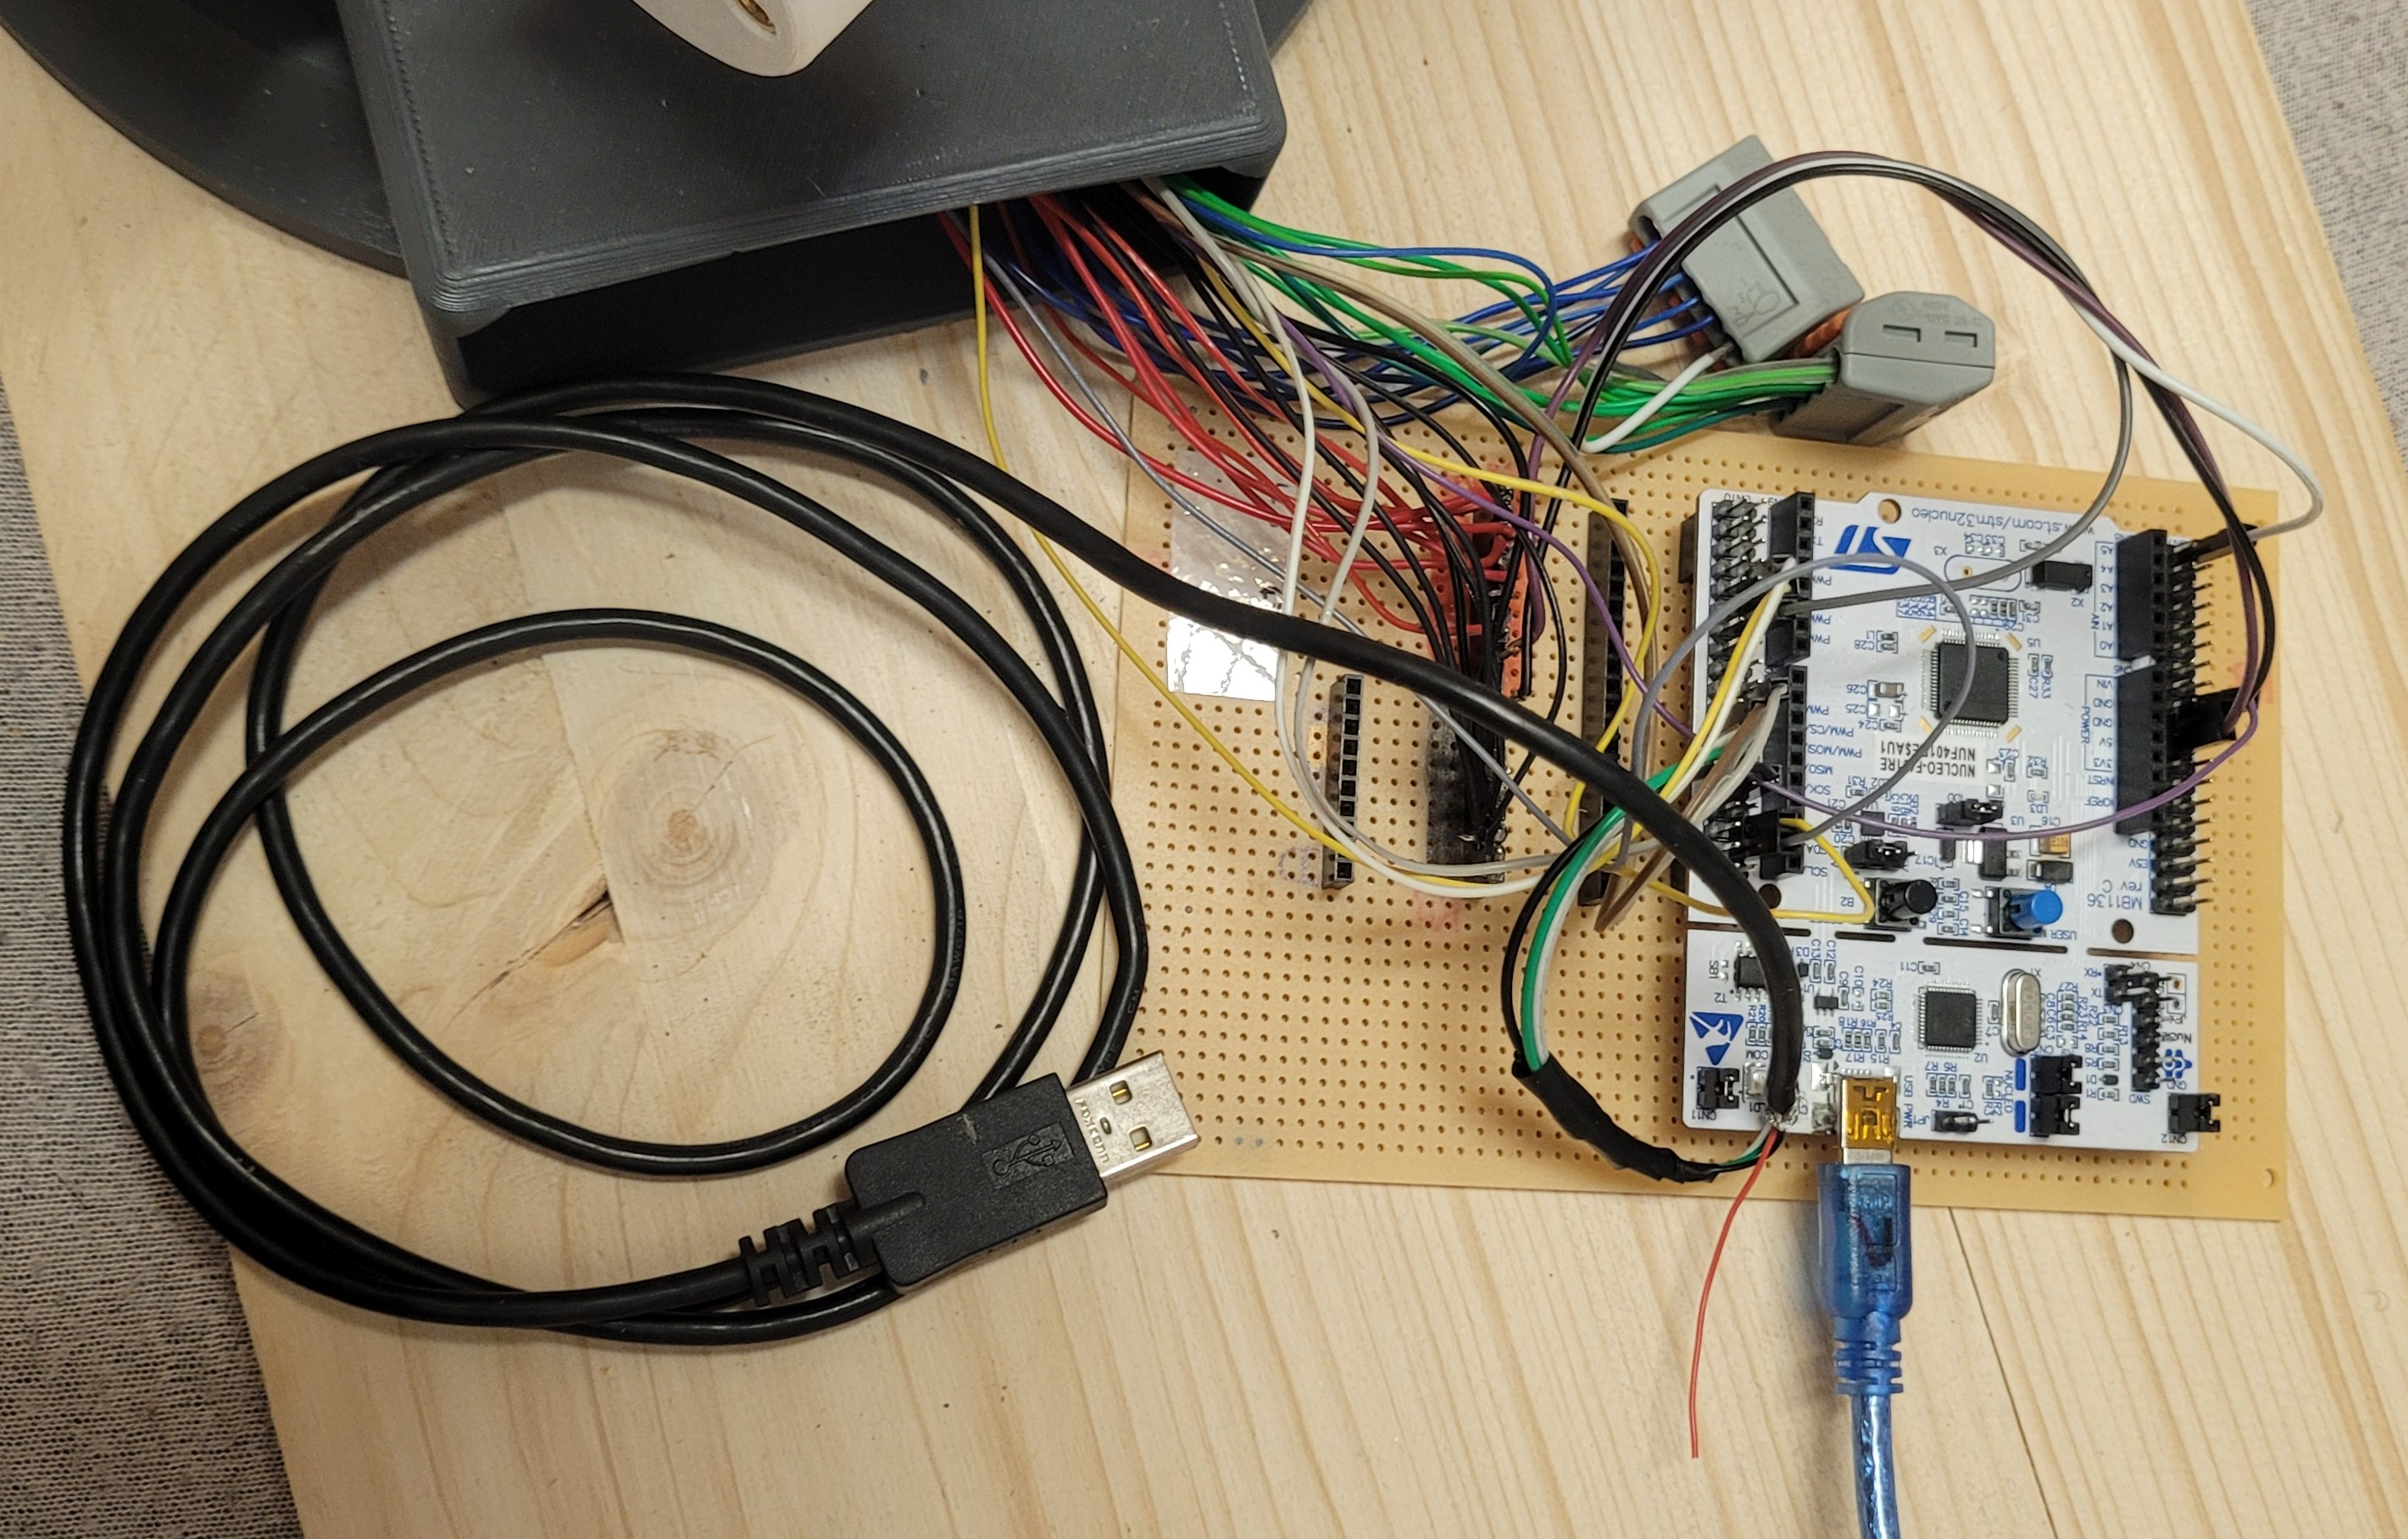
\includegraphics[width=100mm, keepaspectratio]{figures/Csuklo_szog_teszt/mikrovez_2}
\caption{Az összeállított rendszer}
\label{fig:szummarendszer}
\end{figure}


\newpage
\subsection{GMR szenzorok tesztelése}

A következő képeken dokumentáltam a szenzorok egyenkénti működését.

\begin{figure}[!ht]
\centering
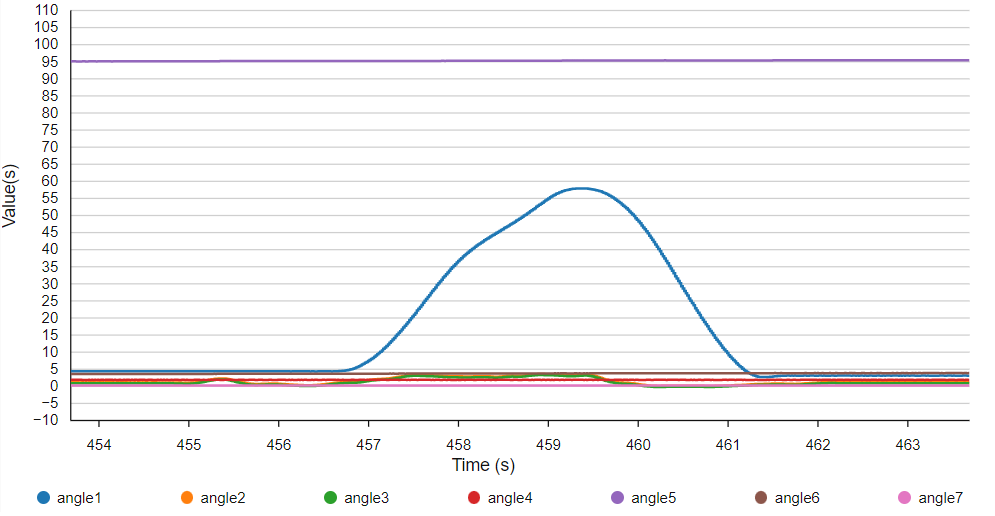
\includegraphics[width=100mm, keepaspectratio]{figures/Csuklo_szog_teszt/1}
\caption{Az első csuklóban található szenzor tesztje}
\label{fig:csuklo_teszt_1}
\end{figure}

\begin{figure}[!ht]
\centering
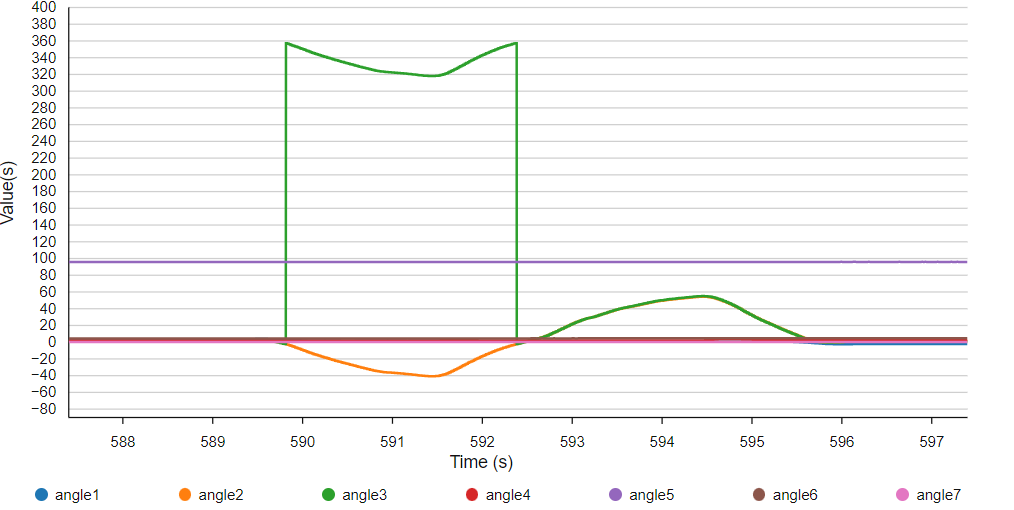
\includegraphics[width=100mm, keepaspectratio]{figures/Csuklo_szog_teszt/2_3}
\caption{Az második csuklóban található szenzor tesztje}
\label{fig:csuklo_teszt_2_3}
\end{figure}

\begin{figure}[!ht]
\centering
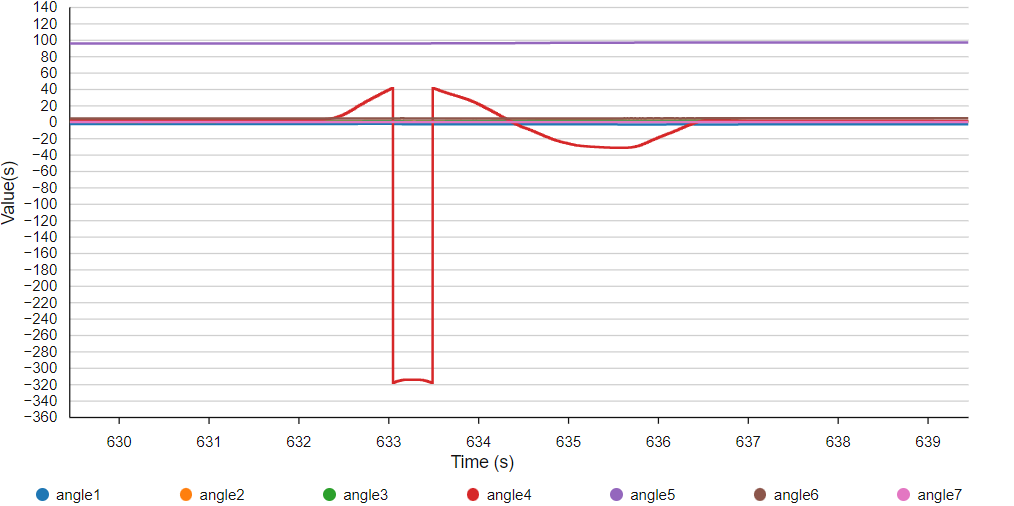
\includegraphics[width=100mm, keepaspectratio]{figures/Csuklo_szog_teszt/4}
\caption{Az harmadik csuklóban található szenzor tesztje}
\label{fig:csuklo_teszt_4}
\end{figure}

\begin{figure}[!ht]
\centering
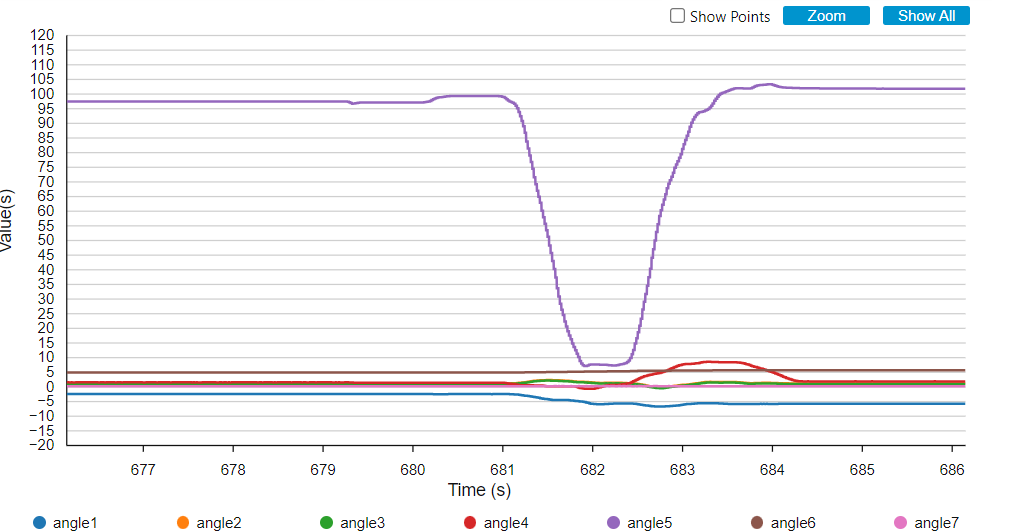
\includegraphics[width=100mm, keepaspectratio]{figures/Csuklo_szog_teszt/5}
\caption{Az negyedik csuklóban található szenzor tesztje}
\label{fig:csuklo_teszt_5}
\end{figure}

\begin{figure}[!ht]
\centering
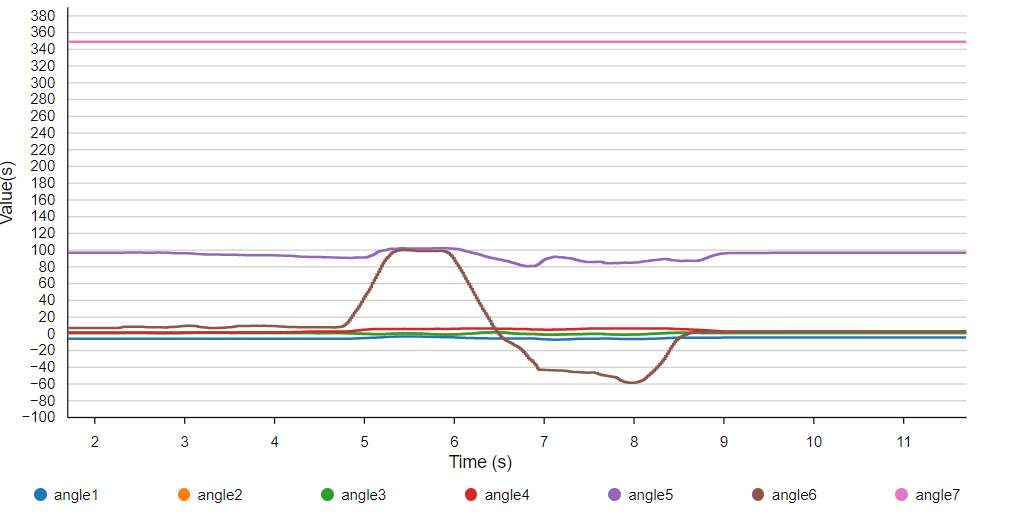
\includegraphics[width=100mm, keepaspectratio]{figures/Csuklo_szog_teszt/6}
\caption{Az ötödik csuklóban található szenzor tesztje}
\label{fig:csuklo_teszt_6}
\end{figure}

\begin{figure}[!ht]
\centering
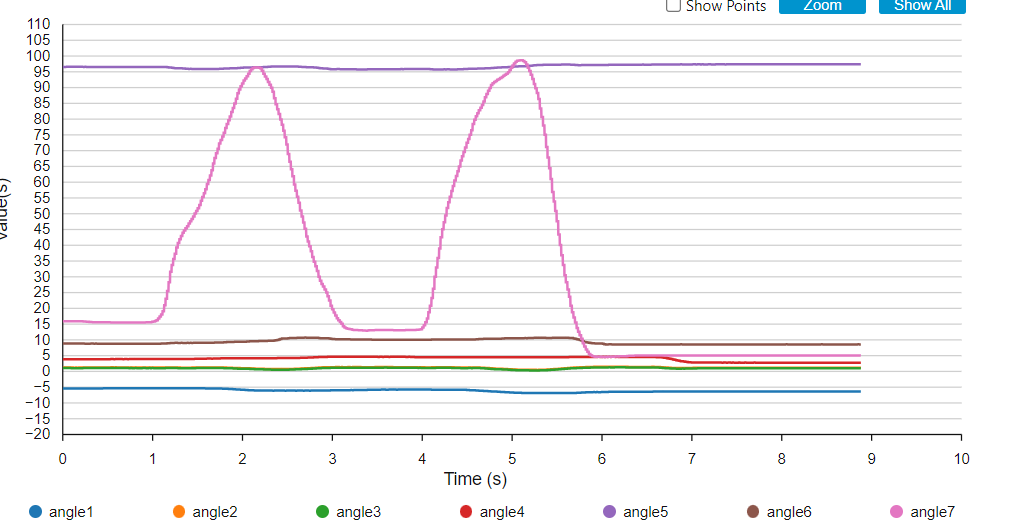
\includegraphics[width=100mm, keepaspectratio]{figures/Csuklo_szog_teszt/7}
\caption{Az hatodik csuklóban található szenzor tesztje}
\label{fig:csuklo_teszt_7}
\end{figure}

\begin{figure}[!ht]
\centering
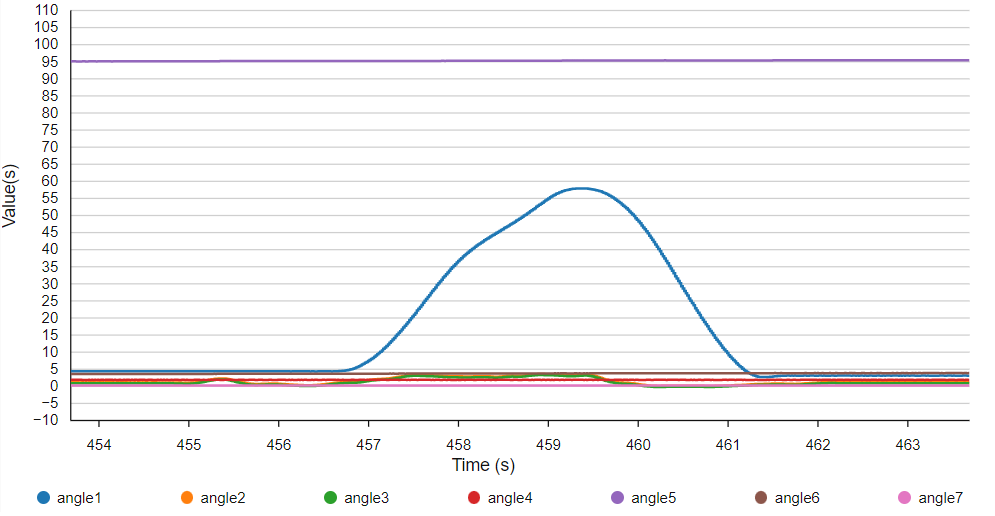
\includegraphics[width=100mm, keepaspectratio]{figures/Csuklo_szog_teszt/1}
\caption{Az első csuklóban}
\label{fig:csuklo_teszt_1}
\end{figure}

Minden szenzor tökéletesen működik. A csukló szöge néhol azért léphetik át a negatív félsíkre, mert a szenzor üzembe helyezés pillanatában, még az offeszetelés nem volt tökéletesen implementálva. Az offszetelést némiképpen pontosabban is lehetne végezni, de ez még a robot használatának szempontjából nem fatális hiba.


\subsection{Vezeték ellenállás mérése}

A vezeték hosszának figyelembe vételével azért szerettem volna foglalkozni, mert az egyik tovább fejlesztési lehetőség amit szeretnék megvalósítani vezeték nélkül kötné össze a telemanipulátort a robot vezérlővel (XYZ fejezet). A vezeték nélküli kommunikáció, ugyan a mikrovezérlő után valósulna meg és nem a szenzor és a közte. Úgy vélem meggyőződni, hogy mekkora lehet a maximális vezeték amit használatok a telemanipulátoron mindenképpen fontos, mert így a impedanciák és interferenciákból fakadó hibákat, illetve továbbfejlesztés esetében figyelembe tudom venni.


%----------------------------------------------------------------------------
%----------------------------------------------------------------------------
       % 4. fejezet
\chapter{Telemanipulátor programja}
\label{sec:LatexTools}

Az telemanipulátor jelfeldolgozó rendszerének fizikai összeállítása után a szenzorok által küldött jelek szoftveres feldolgozását és használatát mutatom be. A fejezet során hasonlóan mint korábban a szenzoroktól kezdem a szoftveres komponensek bemutatását és haladok a tényleges robot mozgatásra szolgáló rendszerekig.

%----------------------------------------------------------------------------
\section{Szenzor kommunikációs protokollja}
%----------------------------------------------------------------------------
A GMR szenzor a mikrovezérlővel az úgy nevezett Synchronous Serial Communication \footnote{magyarul Szinkron Szériás Kommunikációs} röviden SSC protokolt használ. Ez a  protokoll egy olyan kommunikációs rendszer, amely során a küldő és a fogadó eszközök szorosan szinkronizáltak egymással a közös órajel alapján. Az SSC azon alapul, hogy mindkét eszköz előre rögzített órajelet használ a bekapcsolás pillanatától, hogy a rendszer használat teljes ideje alatt szinkronban maradjanak.

A protokoll közös órajele biztosítja, hogy a adat transzferálás esetén az órajel biztosítja, hogy mindkét eszköz azonos sebességgel és időzítéssel küldje és fogadja az üzenetet. Ez az információ küldés során bitek sorozataként továbbítódik, és a kommunikáló fogadó és küldő egységek egyeztetik az adatok kezdőpontját és végpontját az órajelet használva. Ennek következtében mindkét eszköz tudja, hogy mikortól kell és meddig értelmeznie az érkező biteket.

%TODO kép a GMR bitekről

A protokoll lehetővé teszi a teljes és a fél-duplex kommunikációt. Teljes-duplex esetén mindkét eszköz képes egyszerre küldeni és fogadni adatokat, míg fél-duplex esetén a kommunikáció váltakozva történik, azaz egyik eszköz küld, majd vált, és a másik eszköz fogad.

Az SSC gyakran használt alkalmazása az I2C (Inter-Integrated Circuit) és a SPI (Serial Peripheral Interface) kommunikációs protokollok. Az I2C esetén a kommunikáció két vezetéken, adatazon és órajelező vonalon történik, míg az SPI esetén több vezetéket használnak, például MISO (Master In Slave Out), MOSI (Master Out Slave In), órajeladóval és választóvonal.

A SSC protokoll széles körben alkalmazható az elektronikában és beágyazott rendszerekben, ahol szükség van a gyors, megbízható és szinkronizált adatkommunikációra a különböző eszközök között.

A telemanipulátor esetében half-duplex kommunikációs módot használok a GMR szenzor dokumentációjában meghatározott értéken (XYZ hivatkozás) állítottam be. Minden szenzorhoz tartozóan chipválasztó pineket is deklarálnom kellett. A kommunikációs protokoll kezeléséhez egy előre elkészített könyvtárat használtam, ami megtalálható a (XYZ melléklet) mellékletben.


\section{Mikrovezérlő program}
%----------------------------------------------------------------------------

A mikrovezérlő program a diploma dolgozathoz képest kisebb módosításokkal lett kiegészítve, de igazán nagy fejlesztést nem igényelt a program. A elvárásoknál támasztott elvárásoknak megfelelt. Kellően gyors és könnyen módosítható lett. (Fejezet hivatkozás XYZ)

A telemnanipulátornál használt program a konzulensem által készített hasonlóelven működő haptikus vezérlőjének(Hivatkozás XYZ) a mikrovezérlő programját vettem alapul. A programot gyorsan a saját eszközömhöz szükséges módosításokkal eltudtam látni, mivel ez az is STM32-es rendszerre lett készített.

Főkülönbségek, hogy a mikrovezérlő az én általam használt telemanipulátor esetében 7 szenzor adatait gyűjti össze, dolgozza fel és továbbítja a további rendszereknek.

A mikrovezérlő programba implementált funkciók a következők:

\begin{itemize}
\item Szögérték kiolvasás
\item Szögérték offszetelés
\item Szögérték Kinemtaikailag felvett forgás tengelyre igazítása
\item Szögértékek tömbértékek összegyűjtése
\item Kommunikáció a mikrovezérlőhöz csatlakoztatott számítógéppel
\end{itemize}

A szögértékeket szekvenciálisan az $1.$ csukló szenzortól a $7.$ csukló szenzorig egymásután olvassa ki. A szenzor kommunikáció már a bemutatott SSC kommunikáción történik és minden szenzor saját chipselect pin-jének a jelváltozására\footnote{A TLE 5012B GMR szenzor esetében alacsony jelről magas jelre vált a kommunikáció alatt} történik. A kiolvasott szögérték a szenzor meghatározott egyik tengelye és a mágnes kétpólusa által megadott póluspárok egymással bezárt szöge.

%TODO Kép a szenzor szögről.

Az a megkapott szögérték a $-180^\circ$ és $180^\circ$ közötti lehet. Ezt az értéket én át konvertáltam $0^\circ$ és $360^\circ$ fokos skálára ugyan is így sokkal könnyebben beállítható az offset és a forgás irány is egyértelműbb számomra. Az offszet paraméterek beállítása a program indulása után is változtatható, de alap paraméterek be vannak égetve. AZ oka ennek, így nem kellett minden tesztelési ciklus elején offszetelnem. A offszet értékeket a következő képpen állapítottam meg.

\begin{enumerate}
  \item Minden csuklón van egy jelző egyenes, ami a két tengely koordináta rendszereinek a párhuzamosságát jelenti abban az állásban
  \item A kinematikai felírásban vett koordináta rendszer szerinti nullába mozgattam a megfelelő csuklót
  \item Kiolvastam a szenzor adott pontú értékét
  \item Ha pozitív előjelű volt akkor kivontam, ha pedig negatív akkor hozzáadtam a kiolvasott értékhez az offszetet
\end{enumerate}

Az így megkapott szögértékek elfordulására kell még figyelni. Ugyanis a szenzor és mágnes elhelyezkedése a tengelyen befolyásolja, hogy a szögéréték a tengely körüli elfordulással melyik irányba pozitív. Ha a forgatási irány eltér egyszerűen a szögérték mínusz egyszeresét kell venni. 

Ezt követően, ha mindenszögértéket továbbítja a mikrovezérlő, ha igény van rá. Az igényt az interface támasztja a számítógépről még pedig, az UART porton küldött üzenettel. A jelenleg implementált parancsok:

\begin{itemize}
\item $RDS$ - Read from sensor - Szenzor értékek kiolvasás 
\item $KA$ - Keep Alive - Kapcsolat fenntartására vonatkozó parancs
\item $REC$ - Read Error Counter - Hibás kiolvasások darabszámának kiolvasása
\item $CEC$ - Clear Error Counter - Hibás kiolvasás számláló törlése
\end{itemize}

A fenti parancsok közül a REC, CEC és a RDS parancsokat használom. Az RDS esetén a szögértékek kiolvasásra kerülnek és továbbítódnak UART porton, ahogy korábban említettem. A továbbítás egy nagy méretű byte tömben történik, aminek az első két érték amit továbbít egy "OK" és maga az RDS paranccsal megkapott üzenet a többi érték a szenzorokból kiolvasott és számított szögértékek. A REC és a CEC parancsot a szenzorok üzembe helyezésekor használtam. Egy egyszerű port terminál kezelését lehetővé tévő programmal csatlakoztam a mikrovezérlőre és elküldtem a RDS parancsot kétszer. A két kiadott parancs között megváltoztattam a telemanipulátor orientációját. A beüzemelés alatt, több szenzor se működött azonnal és a CEC és REC parancsokkal tudtam a hiba darabszám tárolókat kiolvasni és törölni. A továbbiakban szeretnék még offszet érték beállítására vonatkozó metódust implementálni, illetve jelrögzítést és offszet-be állásra vonatkozó parancsokat.

A mikrovezérlő programmal kapcsolatban nagyon fontos még kitérni a RTOS (XYZ hivatkozás) rendszerre. Ez a STM32 vezérlőknél elérhető funkció a real-timehoz nagyon közeli működést tesz lehetővé. A program így előre megjósolható és determinisztikus módon válaszol az eseményekre, ugyanis realtime rendszerekben a feladatoknak szigorú időkorlátoknak kell megfelelniük, és az RTOS biztosítja a prioritáskezelést, időosztást és egyéb funkciókat a hatékony valós idejű működés érdekében.

%TODO rtos kép

A kritériumokban(XYZ) meghatározott $4[ms]$ vagy gyorsabb lefutás a robot vezérlés eléréséhez nagyban hozzájárul ez a lehetőség. A RTOS-sel elérhető párhuzamos lefutószerű működés és a szigorúan definiált feladatok a mikrovezérlő szögérték kiolvasási feladatát biztosítja, hogy megfelel a kritériumoknak.

\section{Haptikus interfész}
%----------------------------------------------------------------------------

A mikrovezérlő a számítógéphez, amin ez az interface fut UART porton(XYZ fejezet) csatlakozik. A telemanipulátor csuklóiban mért szenzor jeleket a haptikus interface kéri el a mikrovezérlőtől. A haptikus jelző ebben az esetben azt jelenti, hogy visszajelzés is van építve a rendszerbe. A sikeres megfogás vagy ütközés esetén a haptikus interface képes a openmanipulátor (XYZ melléklet) vezérlő telemnanipulátorába épített rezgő motoroknak jelet adni. Az általam készített telemanipulátorba nincs ilyen típusú visszajelzés beépítve. Az interface ezt a visszajelzési visszacsatolást leszámítva tökéletesen megfelel az általam kitűzött célnak. Ezt a szoftveres megoldást annak ellenére, hogy nem egy az egyben a saját munkám fontosnak tartom bemutatni, hogy a tovább fejlesztési lehetőségeknél kitudjak arra térni, hogy miért lenne fontos ezt az eszköz interfacet tovább módosítani és fejleszteni.

Az interface két részre bontható. Az első az, ami megvalósítja a kommunikációt a mikrovezérlővel a másik pedig egy ROS node, ami a telemanipulátorból kiolvasott szögjeleket publikálja. Az szerial kommunikáció egy egyszerű "USB"-s csatlakozásnak minősül, ami azt jelenti, hogy lehetőség van információt küldeni és kiolvasni a port-ról. A csatlakoztatott mikorvezérlő a fizikai porton jelenik meg a számítógép port listájában Linuxon ez a $tty*$ portok között van. Fontos megjegyezni, hogy a teljes dolgozatom Ubuntu vagy közimsertebb nevén Linux operációs rendszeren lett megvalósítva. Windows operációs rendszeren is van lehetőség futtatni, ebben az esetben viszont virtuális gépet\footnote{Olyan programok amelyek képesek Windows operációs rendszeren telepített programban valamilyen nem Windows környezetre készített programot futtatni} vagy Windows Subsystem for Linux\footnote{Microsoft által támogatott virtuális Linux operációs rendszer. A egyik legelterjedtebb megoldás arra, hogy Windows operációs rendszerrel rendelkező eszközökön Linux-ot futassunk} - rövidítve WSL - kell használni. Természetesen számos más megoldás van, mint például a dual-Boot\footnote{Linux és Windows operációs rendszerek ugyanazon eszközön egymás mellé a háttértárba fel vannak telepítve és a számítógép elindulásánál lehet megválasztani, hogy melyiket akarjuk indítani. Ebben az esetben sokkal kiegyensúlyozotabb hardver terhelést kapunk és teljes értékű operációs rendszerekkel dolgozunk, ami a stabilitást nagy mértékben javítja.}. Én a diploma dolgozatomban bemutatott telemanipulátor esetében teljesértű Linux operációs rendszerrel ellátott illetve dual-Bootos számítógépet használtam.

A fizikai szerial kommunikáció létrejötte utána az interfacenek ugyanazok a kommunikációs paraméterek lettek beállítva, mint amit a mikorvezérlő is használ. Ez triviális ugyanis, ahogy a XYZ fejezetben bemutattam a UART prtokolt fontos, hogy a két eszköz szinkronban legyen. A beállított paraméterek:

\begin{itemize}
\item Baudrate (Kommunikáció sebessége) - $115200 [-]$
\item Paritás Bit (Hibajelző bit) - Nincs
\item Stop bit szám - $1 [db]$
\item Byte méret - $8[db]$
\end{itemize}

Ezzel létrejött a programban is használható kommunikációs kapcsolat a számítógép és a mikrovezérlő között. Az interface ezt követően ciklikusan $8[ms]$-onként a kommunikációs porton az RDS parancs segítségével lekérdezi a csuklószögeket. A visszakapott választ ellenőrzi, hogy az előző fejezetben bemutatott sorrendben minden rendben megérkezik-e és így validálva az adatok helyességét. A megkapott csukló szögeket átváltja radiánba és a ROS topológián (XYZ melléklet ros top) is láthatóan publikálja őket.

\section{Universal Robot kontroller}
%----------------------------------------------------------------------------
\section{Gazebo szimuláció}
%----------------------------------------------------------------------------
\section{Valósrobot vezérlése}
%----------------------------------------------------------------------------			 % 5. fejezet
%----------------------------------------------------------------------------
\chapter{\osszefoglalas}
%----------------------------------------------------------------------------

\section{Eredmények}

A diploma dolgozatom elején kitűzött feladatokat maradéktalanul sikerült elvégeznem. Sikeresen elkészítettem egy telemanipulátort, aminek a jelfeldolgozó rendszerével kinematikai számításokat alkalmazva, vezérlési utasításokat tudtam adni egy szimulációs környezetben létrehozott, és egy valós kollaboratív robotnak. Mindkét esetben a vezérlés stabilan fennállt, így folyamatosan tudtam vezérelni a robot és megfigyelni a jelenlegi összeállításom sajátosságait.

Tanulmányaim alatt elsajátított készségek lehetővé tették, hogy a telemanipulátorral kezdeti fizikai világból gyűjtsek szenzorokkal információt a operátor mozgatási szándékáról. Ezt egy zárt szoftveres környezetben robot vezérlési paranccsá alakítsam és ezt továbbítva fizikai világban ezt a robot megvalósítsa ezt.


\section{Tanulságok és tovább fejlesztési irány} 

A telemanipulátor gyakorlatilag minden egyes elemén, amiről a diplomamunkában beszámoltam van lehetőség továbbfejlesztésre.

A telemanipulátor karjainak kialakítását a negyedik és ötödik csukló között át lehet alakítani annak érdekében, hogy a mozgás tartományt ki lehessen használni rugós mechanizmus ellenére is.

A szoftveres rendszerben a szöghibák egységnyi csökkentése vagy egy zajszűrő rendszer illesztése lehetne megfelelő irány, mivel az eredmények alapján nagyon nagy mértékben befolyásolja a szenzorok zaja a robot stabilitását. A további részekben a kontroller kialakítása funkcionális tekintetben is nagy mértékben javítható. Az egész kontroller pálya tervező motorja, illetve a ROS egyes verziójáról a kettesre átállni lehet az egyik legfontosabb cél. Ezzel célkitűzéssel  számtalan új lehetőség kerülne fel a látószögbe és kezdődhetne meg tesztelésük. A szoftveres rendszer legnagyobb és elég általánosnak mondható tanulsága talán, hogy számtalan megoldási lehetőség közül lehet választani és iteratívan tapasztalat szerzéssel lehet csak előre haladni.

Számomra a legnagyobb célkitűzés az lenne, ha egy más gyártó által elérhető robotot is megtudnék vele mozgatni. Erre nem tértem ki a dolgozatomban, de egy KUKA robot mozgatása lehetne a következő mérföld kő, mivel sokkal zártabb vezérlő rendszere van, sokkal kevésbé egyszerűsíthető és megköveteli a valósidejű lefutást.

Egy jövőbe mutató kiegészítés, ha mind ezek vezeték nélkül történnének. Azaz előkészítem a telemanipulátoromat a vezeték nélküli vezérelhetőségre, akár WiFi akár 5G hálózatokon keresztül.

A felsoroltak mellett számtalan módon lehet még ezt a rendszert tovább fejleszteni vagy esetleg új funkciókat hozzáilleszteni.

% Keltezés, aláírás
\vspace{0.5cm}

\begin{flushleft}
{Budapest, \today}
\end{flushleft}

\begin{flushright}
\emph{\authorName}
\end{flushright}

\vfill
           % Összefoglalás


% Bibliográfia [Bibliography]
\addcontentsline{toc}{chapter}{\bibname}
{
    \footnotesize  % Kisebb betűméret [Smaller font size]
    \bibliography{bib/mybib}
}


% Idegen nyelvű (angol) összefoglaló [Foreign language summary]
%----------------------------------------------------------------------------
\chapter*{\summary}\addcontentsline{toc}{chapter}{\summary}
%----------------------------------------------------------------------------

\selectforeignlanguage % angol (magyar) nyelvi beállítások

Az elvégzett munka rövid, másfél oldalt meg nem haladó, de legalább 2/3 
oldalnyi terjedelmű angol nyelvű összefoglalása.

Angol nyelven készített dolgozat esetén magyar nyelvű összefoglaló kell, ha a
készítő magyar anyanyelvű. Nem angol vagy nem magyar nyelven készített
dolgozat esetén kötelező az angol nyelvű összefoglaló, és ha a készítő magyar
anyanyelvű, akkor a magyar nyelvű is.

\vspace{0.5cm}
\paragraph{Keywords} \emph{\keywords}  % A kulcsszavak a fő tex fájlban vannak definiálva


\selectthesislanguage % térjünk vissza magyar (angol) nyelvre



% Függelék és mellékletek [Appendices]
%\excludeFromLocAndLot % A következő ábrákat és a táblázatokat hagyja ki a jegyzékből
                      % [Exclude following figures and tables from List Of Figures/Tables]

%----------------------------------------------------------------------------
\appendix
%----------------------------------------------------------------------------
\chapter*{\fuggelek}\addcontentsline{toc}{chapter}{\fuggelek}
%----------------------------------------------------------------------------
\setcounter{chapter}{\appendixletter} % F betű
%\setcounter{equation}{0}
\numberwithin{equation}{section}
\numberwithin{figure}{section}
\numberwithin{lstlisting}{section}
%\numberwithin{tabular}{section}


% Ismertető - töröld ki
%----------------------------------------------------------------------------
A függelék a főszöveget kiegészíti további részletezéssel. Ide kerül minden kiegészítő információ, ami nem tartozik szorosan a feladat témájához. A függelék rendszerint nem önálló dokumentum. A főszöveg általában nem hivatkozik rá. Általában saját munka.

A dolgozat opcionális eleme, csak igény esetén kell használni.
%----------------------------------------------------------------------------

%----------------------------------------------------------------------------
\section{A TeXstudio felülete}
%----------------------------------------------------------------------------
\begin{figure}[!ht]
\centering
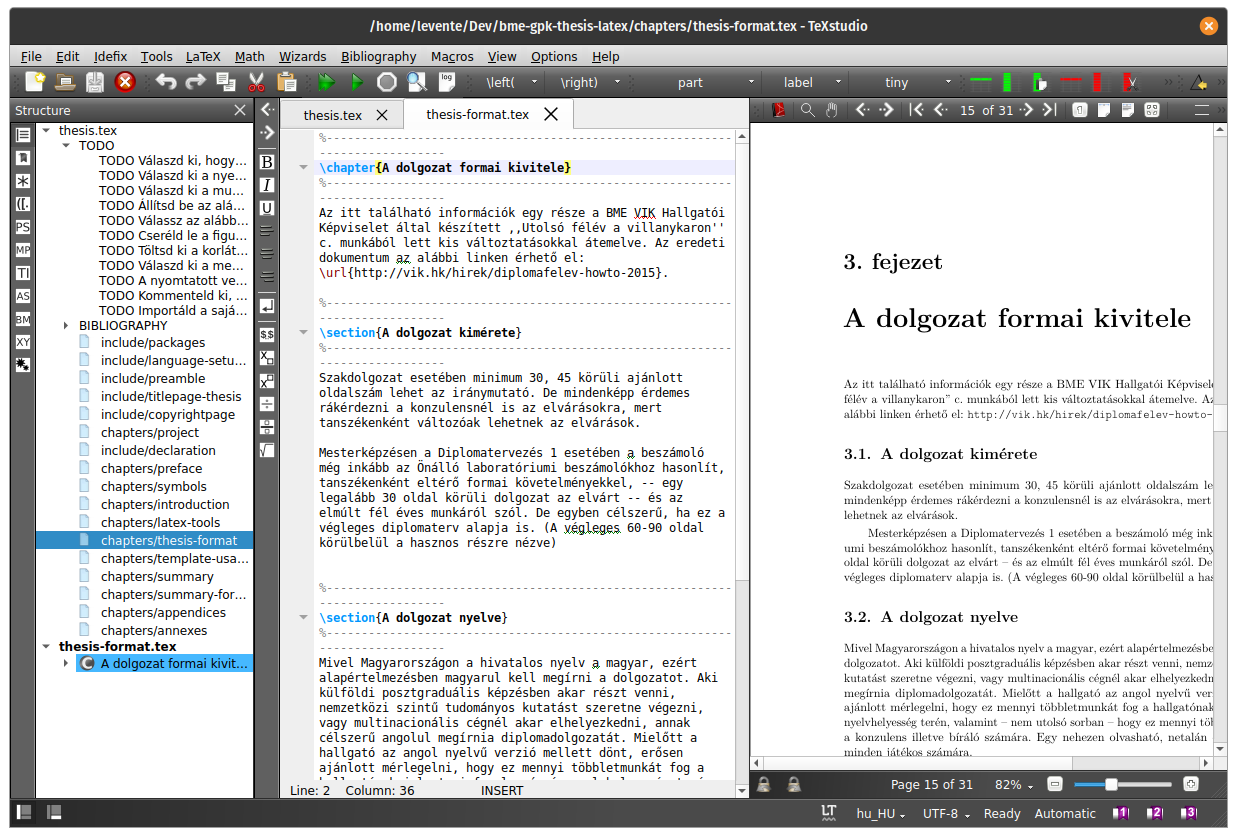
\includegraphics[width=150mm, keepaspectratio]{figures/TeXstudio.png}
\caption{A TeXstudio \LaTeX-szerkesztő.} 
\end{figure}

%----------------------------------------------------------------------------
\clearpage\section{Válasz az ,,Élet, a világmindenség, meg minden'' kérdésére}
%----------------------------------------------------------------------------
A Pitagorasz-tételből levezetve
\begin{align}
c^2=a^2+b^2=42.
\end{align}
A Faraday-indukciós törvényből levezetve
\begin{align}
\rot E=-\frac{dB}{dt}\hspace{1cm}\longrightarrow \hspace{1cm}
U_i=\oint\limits_\mathbf{L}{\mathbf{E}\mathbf{dl}}=-\frac{d}{dt}\int\limits_A{\mathbf{B}\mathbf{da}}=42.
\end{align}
        % Függelék - opcionális
%----------------------------------------------------------------------------
\appendix
%----------------------------------------------------------------------------
\chapter*{\melleklet}\addcontentsline{toc}{chapter}{\melleklet}
%----------------------------------------------------------------------------
\setcounter{chapter}{\annexletter} % M betű
\setcounter{section}{0}
%\setcounter{equation}{0}
\numberwithin{equation}{section}
\numberwithin{figure}{section}
\numberwithin{lstlisting}{section}
%\numberwithin{tabular}{section}

%----------------------------------------------------------------------------
\section{Első melléklet}
%----------------------------------------------------------------------------
           % Mellékletek

\end{document}
